\documentclass[a4paper,12pt,uplatex]{jsarticle}  %%%%%%%%%%%% uplatex
\usepackage{amsmath,amssymb,layout,enumerate,bm,verbatim}
% \usepackage{)  ※パッケージ追加用
\usepackage[dvips,dvipdfmx]{graphicx}  %%%%%%%%%%%%%%%%%%%%%% dvipdfm→dvipdfmx

\setlength{\oddsidemargin}{-15truemm}
\setlength{\topmargin}{-20truemm}
\setlength{\textwidth}{49zw}
\setlength{\textheight}{40\baselineskip}
\addtolength{\textheight}{\topskip}

\setlength{\headheight}{0zw}
\setlength{\headsep}{0zw}

% \setlength{\columnseprule}{0.4pt} % 中央の線の太さの設定
\setlength{\parindent}{0pt}       % 本文の字下げの設定
% \setlength{\mathindent}{4zw}      % 数式の字下げの設定
\setlength{\fboxrule}{0.5pt}      % boxの枠の太さ

\newcommand{\N}{\mathbb{N}}
\newcommand{\Z}{\mathbb{Z}}
\newcommand{\Q}{\mathbb{Q}}
\newcommand{\R}{\mathbb{R}}
\newcommand{\C}{\mathbb{C}}

\newcommand{\ds}{\displaystyle}

\renewcommand{\labelenumi}{(\arabic{enumi})}
% \renewcommand{\labelenumi}{(\roman{enumi})}
% \renewcommand{\labelenumi}{(\theenumi)}
\renewcommand{\theenumii}{\roman{enumii}}

\newcommand{\p}[2]{{}_{#1}\textrm{P}_{#2}}
\renewcommand{\c}[2]{{}_{#1}\textrm{C}_{#2}}
\newcommand{\h}[2]{{}_{#1}\textrm{H}_{#2}}

\pagestyle{empty}

\begin{document}

\section*{数学オリンピックワークショップ 事前演習問題G}

\fbox{G1} (基礎)

\begin{enumerate}
\item 面積18の正六角形$\rm ABCDEF$の内部に点$\rm P$をとるとき,$\triangle {\rm ABP}, \triangle {\rm CDP}, \triangle {\rm EFP}$の面積の和を求めよ。

\item 長さ10の針金を直角に5回折って下の図のような図形を作るとき線分$\rm PQ$の長さの最小値を求めよ。

\begin{figure}[h]
  \centering
  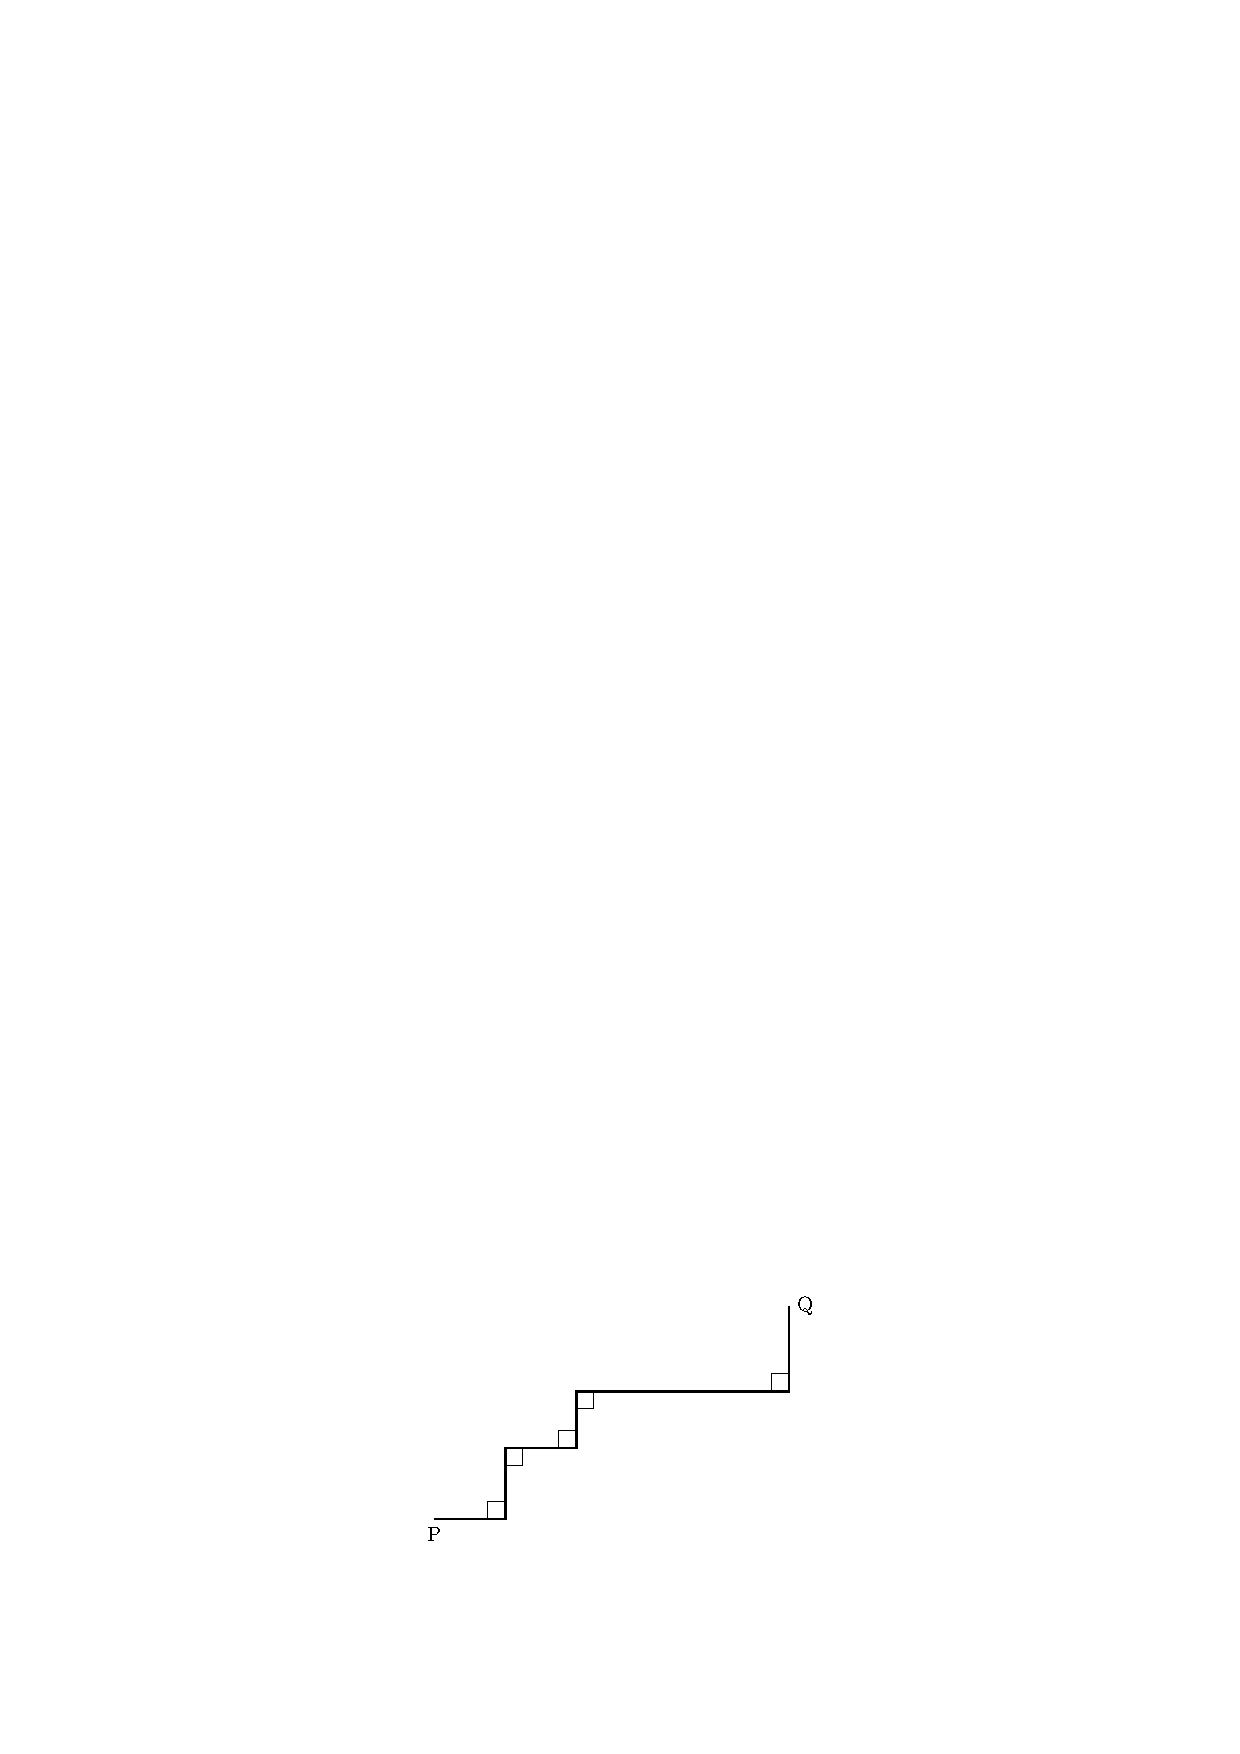
\includegraphics[width=5.0cm]{jizen_1_2_problem.pdf}
\end{figure}


\end{enumerate}

\bigskip

\fbox{G2} (基礎)

\begin{enumerate}
\item 下図のように半径4の円Oの直径AB, CDをとったところ,$\angle {\rm AOC}=30^{\circ}$となった。(劣)弧AD上の点PからAB, CD に下ろした垂線の足をそれぞれX, Yとするとき,線分XYの長さを求めよ。

\begin{figure}[h]
  \centering
  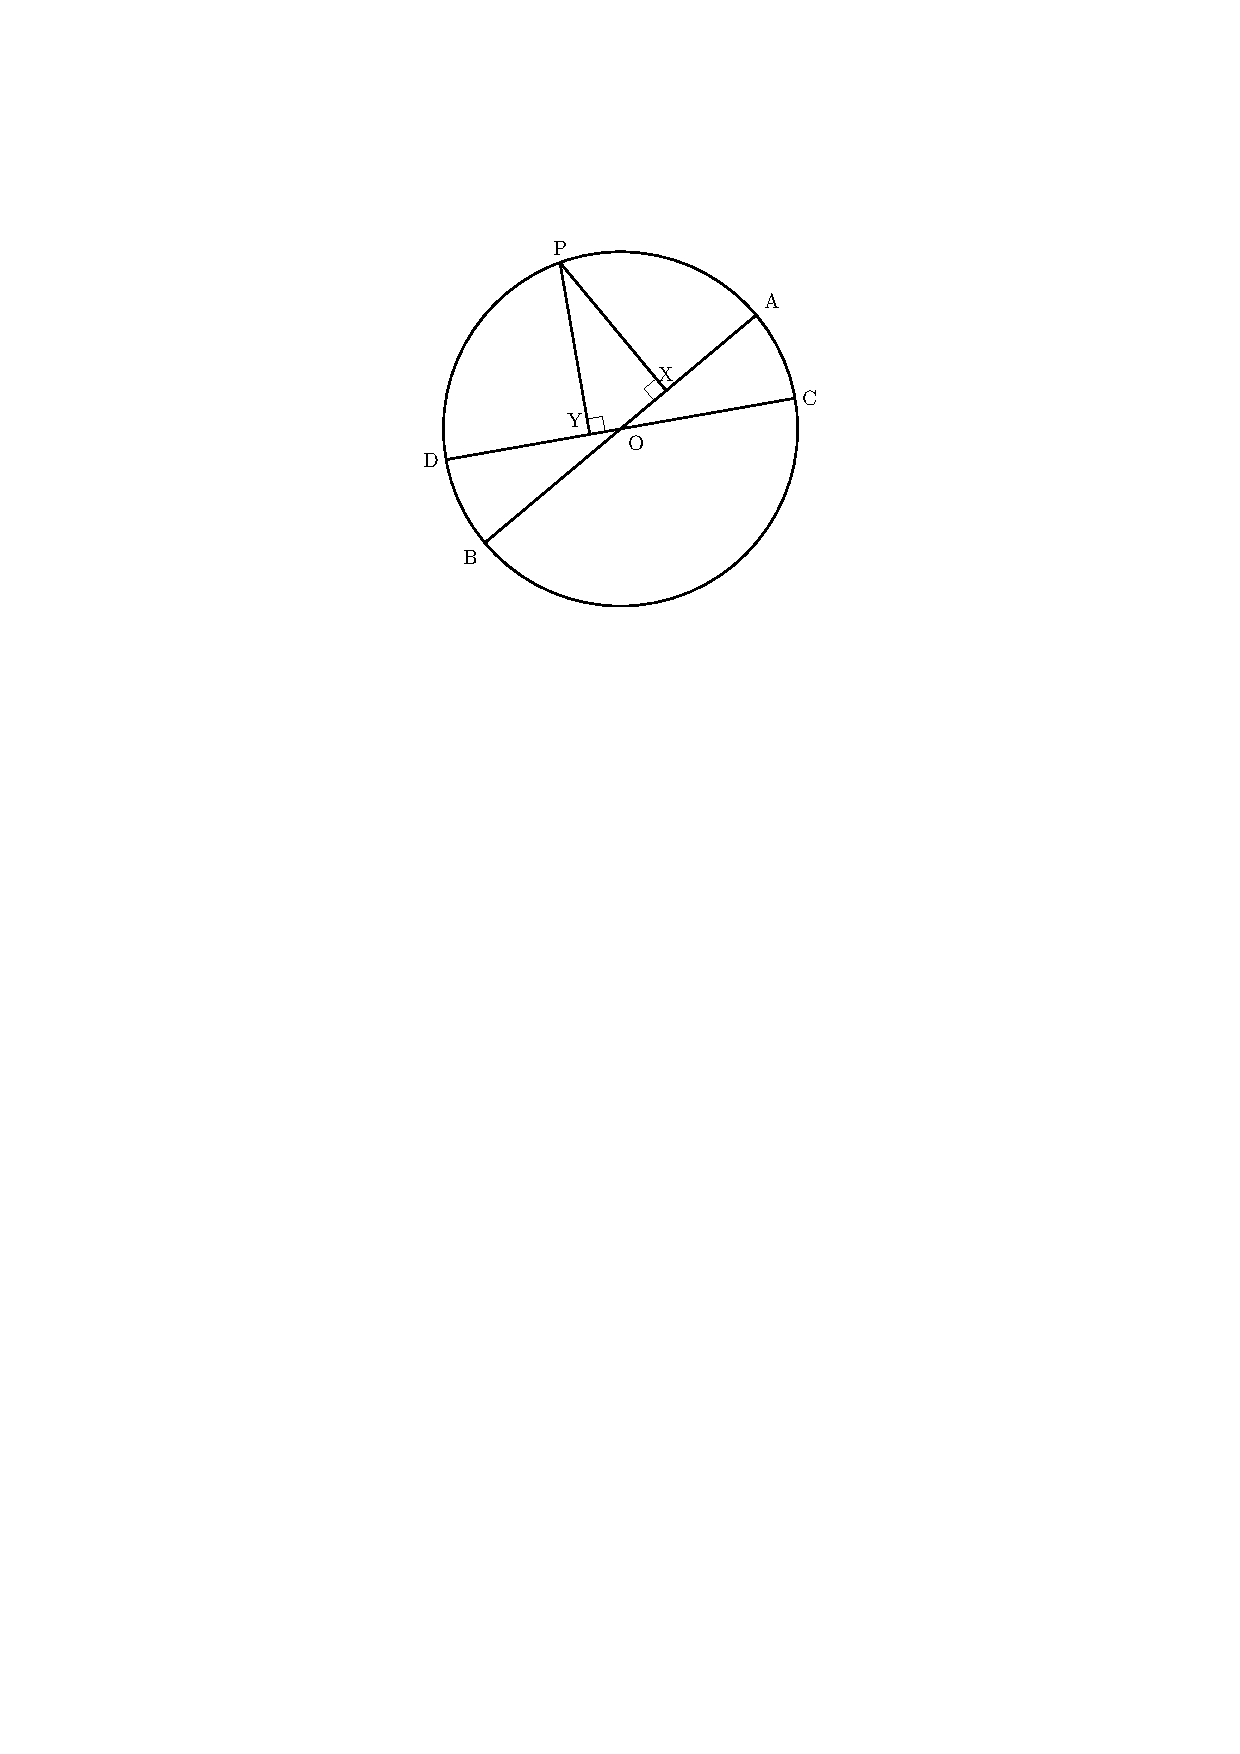
\includegraphics[width=5.0cm]{jizen_2_1_problem.pdf}
\end{figure}

\item 六角形ABCDEFは円に内接しており,またAD, BE, CFは一点Pで交わっている。${\rm AB}=3, {\rm BC}=4, {\rm CD}=5, {\rm DE}=6, {\rm EF}=9$のとき,FAの長さを求めよ。

\begin{figure}[h]
  \centering
  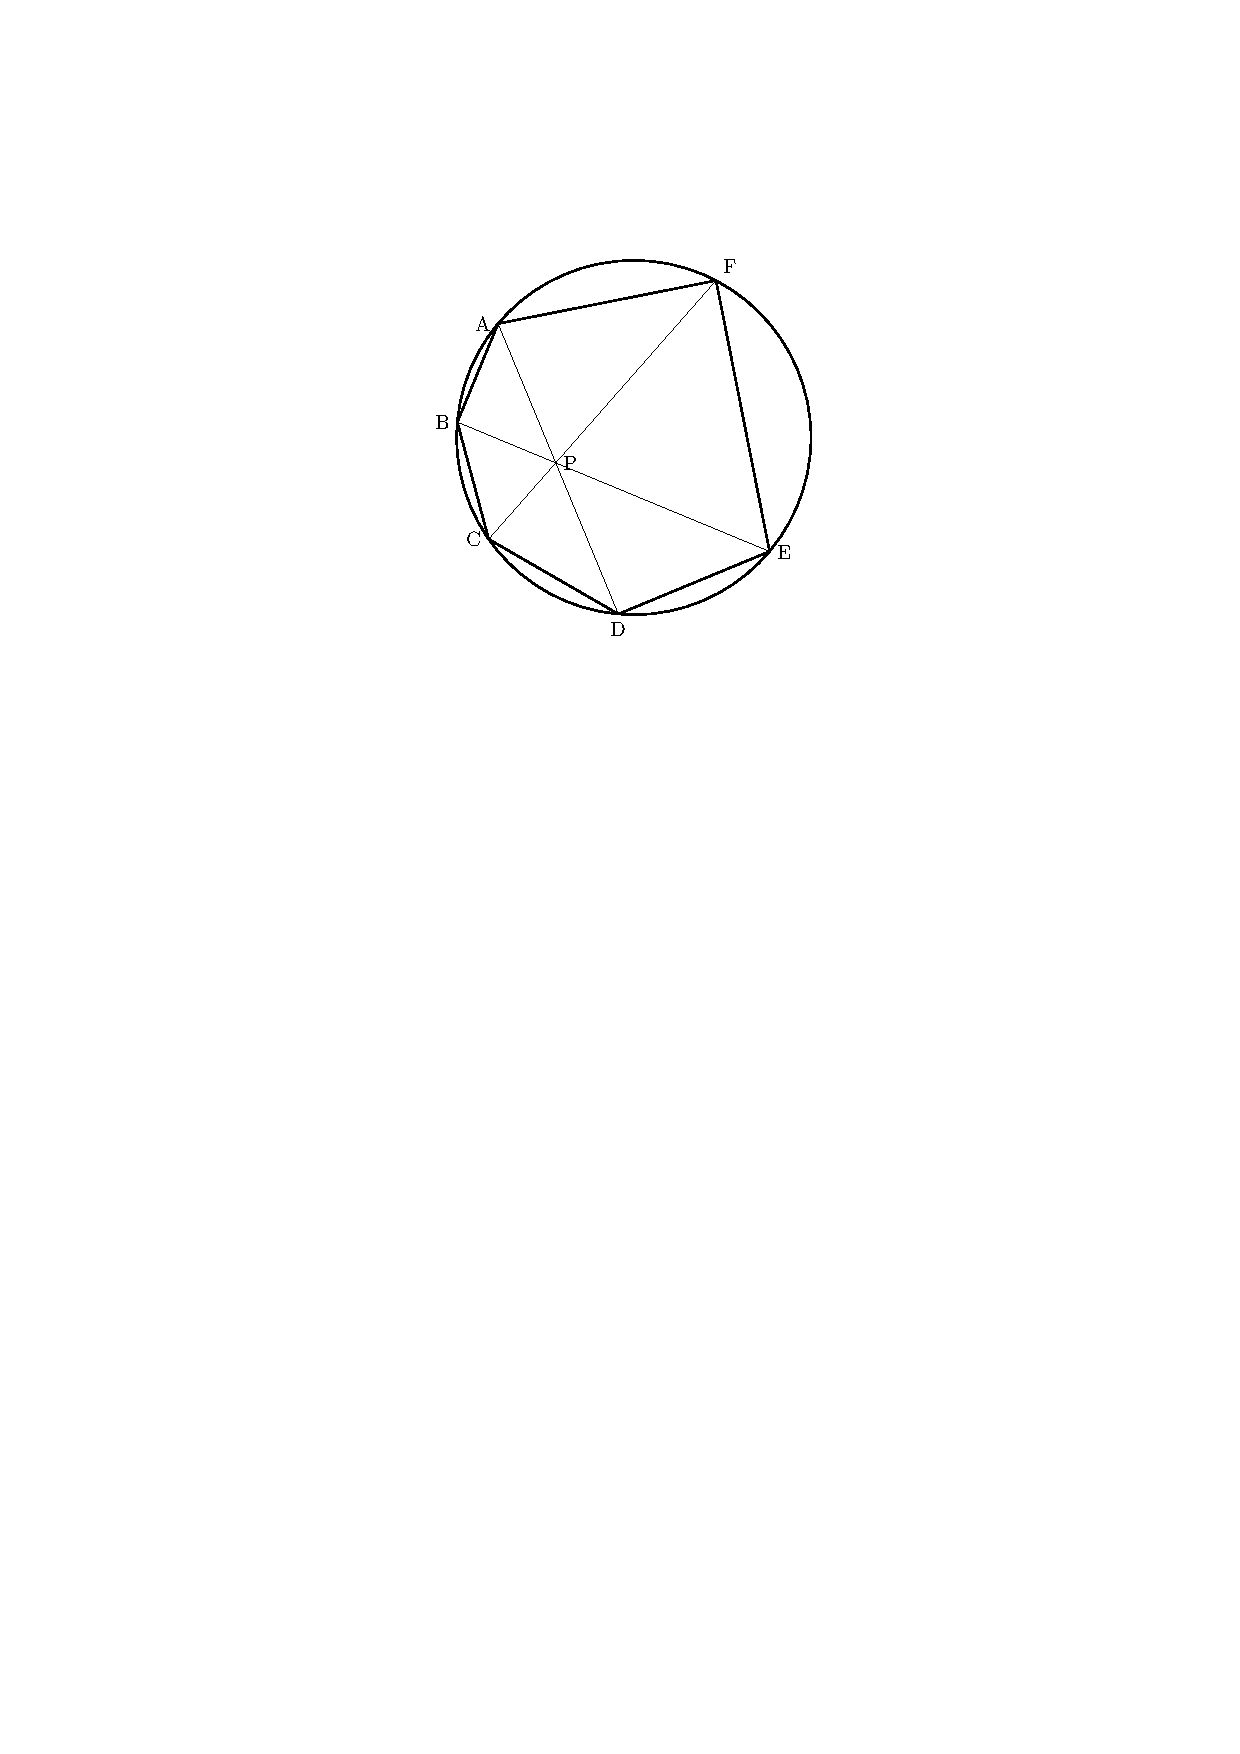
\includegraphics[width=5.0cm]{jizen_2_2_problem.pdf}
\end{figure}

\end{enumerate}

\bigskip

\fbox{G3} (標準)(高校生向け)

\begin{enumerate}
\item 正の実数$x, y, z$が以下の関係式を満たすとき$xy+\dfrac{\sqrt 3}{2}yz+\dfrac{1}{2}zx$の値を求めよ。

\begin{equation}
  \left\{
    \begin{alignedat}{1}
      &x^{2} + y^{2} =9 \\ 
      &y^{2} +yz+z^{2} = 25   \\
      &z^{2} + \sqrt{3}zx + x^{2} = 16  \nonumber
    \end{alignedat}
  \right.
\end{equation}


\item 実数$a,b,c,d,e,f,g,h$に対して,$ac+bd, ce+df, eg+fh, ga+hb, ae+bf, cg+dh$のうち少なくとも1つは0以上であることを示せ。
\end{enumerate}

\bigskip

\fbox{G4} (標準)

\begin{enumerate}
\item 正四角錐$\rm O-ABCD$に対して平面$\alpha$が辺$\rm OA, OB, OC, OD$とそれぞれ点$\rm P, Q, R, S$で交わっている。$\rm OP=2, OQ=4, OR=3$のとき,$\rm OS$の長さを求めよ。
\item 正方形ABCDについて,ACとBDの交点をOとし,線分OA,OB,OC,OD上にそれぞれ点P,Q,R,Sをとる。QRとBC, PQとAB, RSとCDの交点をX,Y,Zとしたところ,これらは同一直線上にあった。$\rm OP=2, OQ=4, OR=3$のとき,$\rm OS$の長さを求めよ。

\begin{figure}[ht]
  \centering
  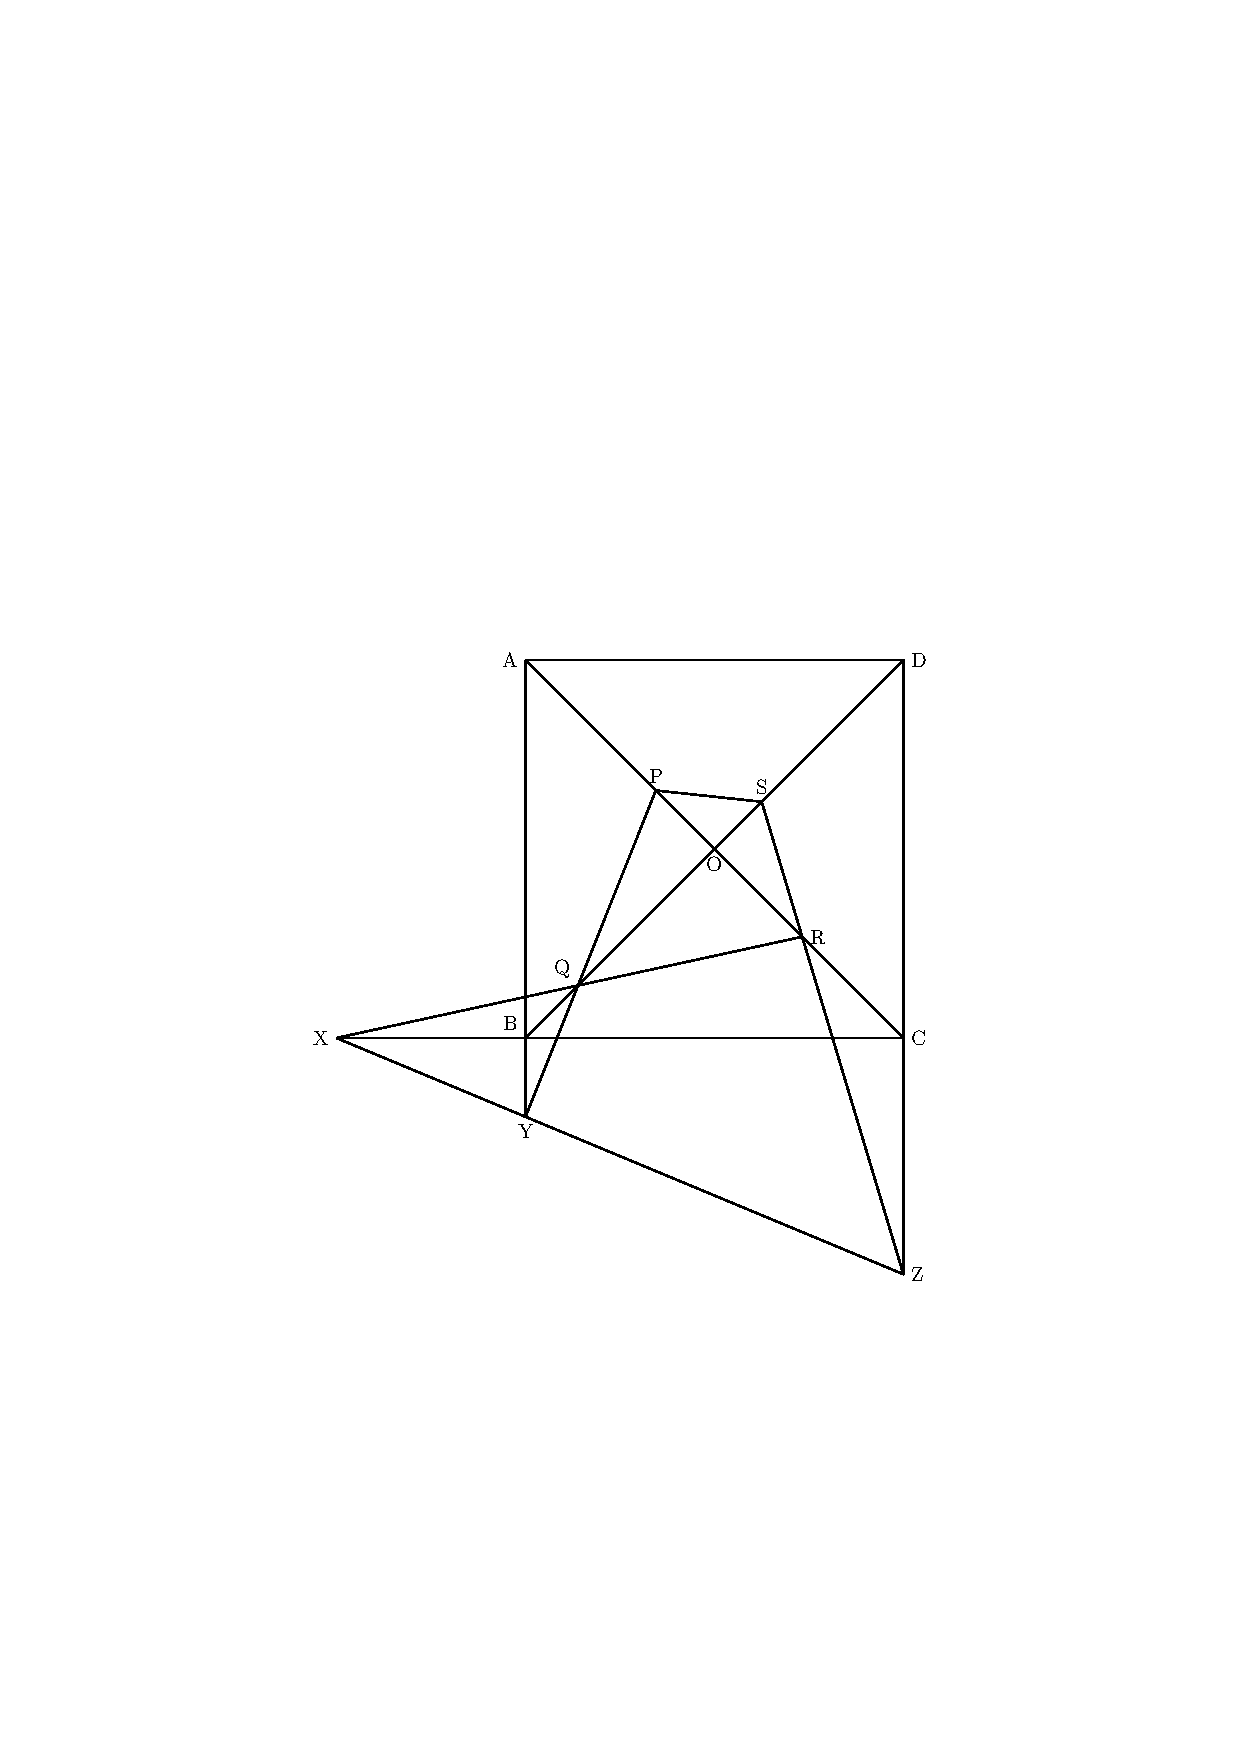
\includegraphics[width=8.0cm]{jizen_4_2_problem.pdf}
\end{figure}

\end{enumerate}

\bigskip

\newpage

\fbox{G5} (応用)

\begin{enumerate}
\item $\triangle {\rm ABC}$の外接円のB, C における接線の交点をDとする。BCの中点をMとするとき,$\angle{\rm BAM} = \angle{\rm CAD}$であることを示せ。

\begin{figure}[ht]
  \centering
  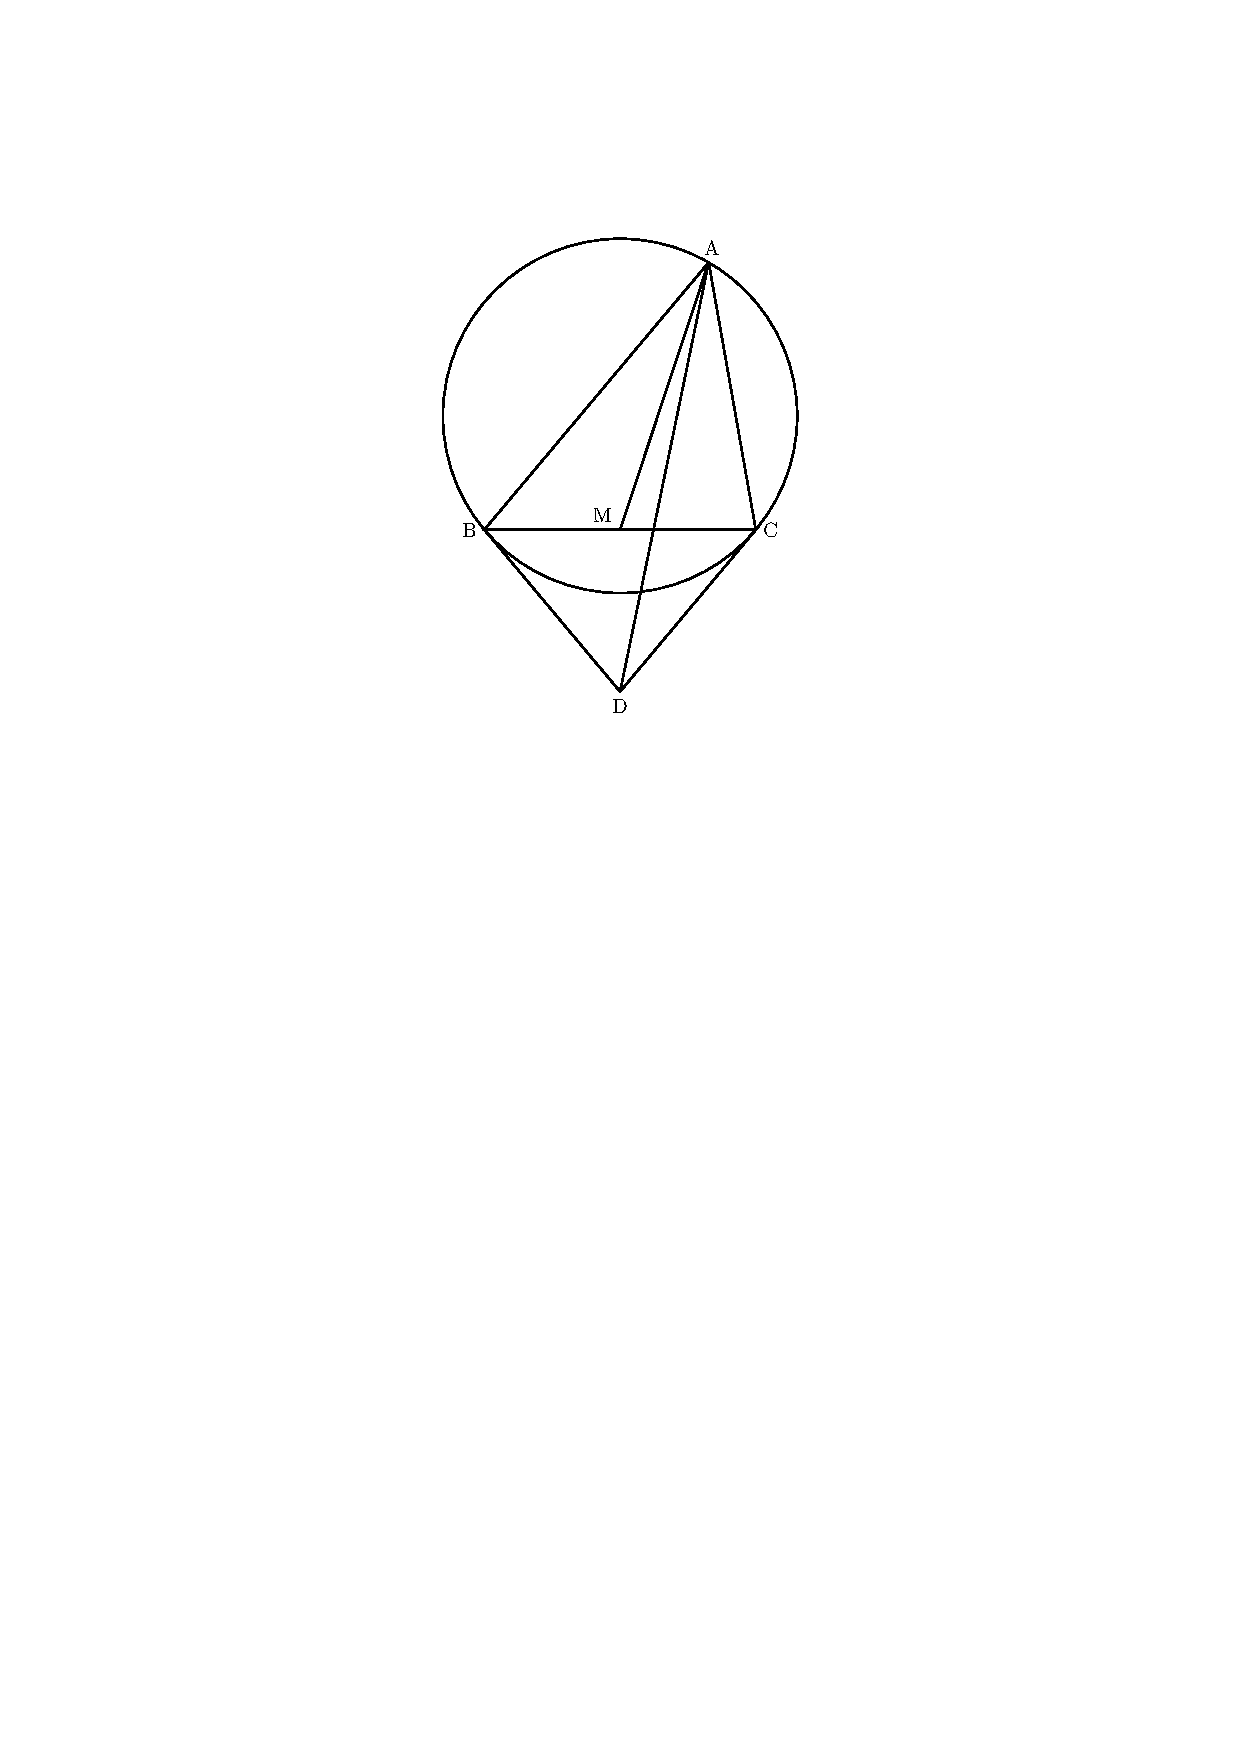
\includegraphics[width=6.0cm]{jizen_5_1_problem.pdf}
\end{figure}

\item $\rm AB=AC$なる$\triangle {\rm ABC}$の内部に点Pをとったところ,$\angle{\rm PBA} = \angle{\rm PCB}$となった。BCの中点をMとするとき,$\angle{\rm APC} + \angle{\rm BPM}=180^{\circ}$であることを示せ。


\begin{figure}[h]
  \centering
  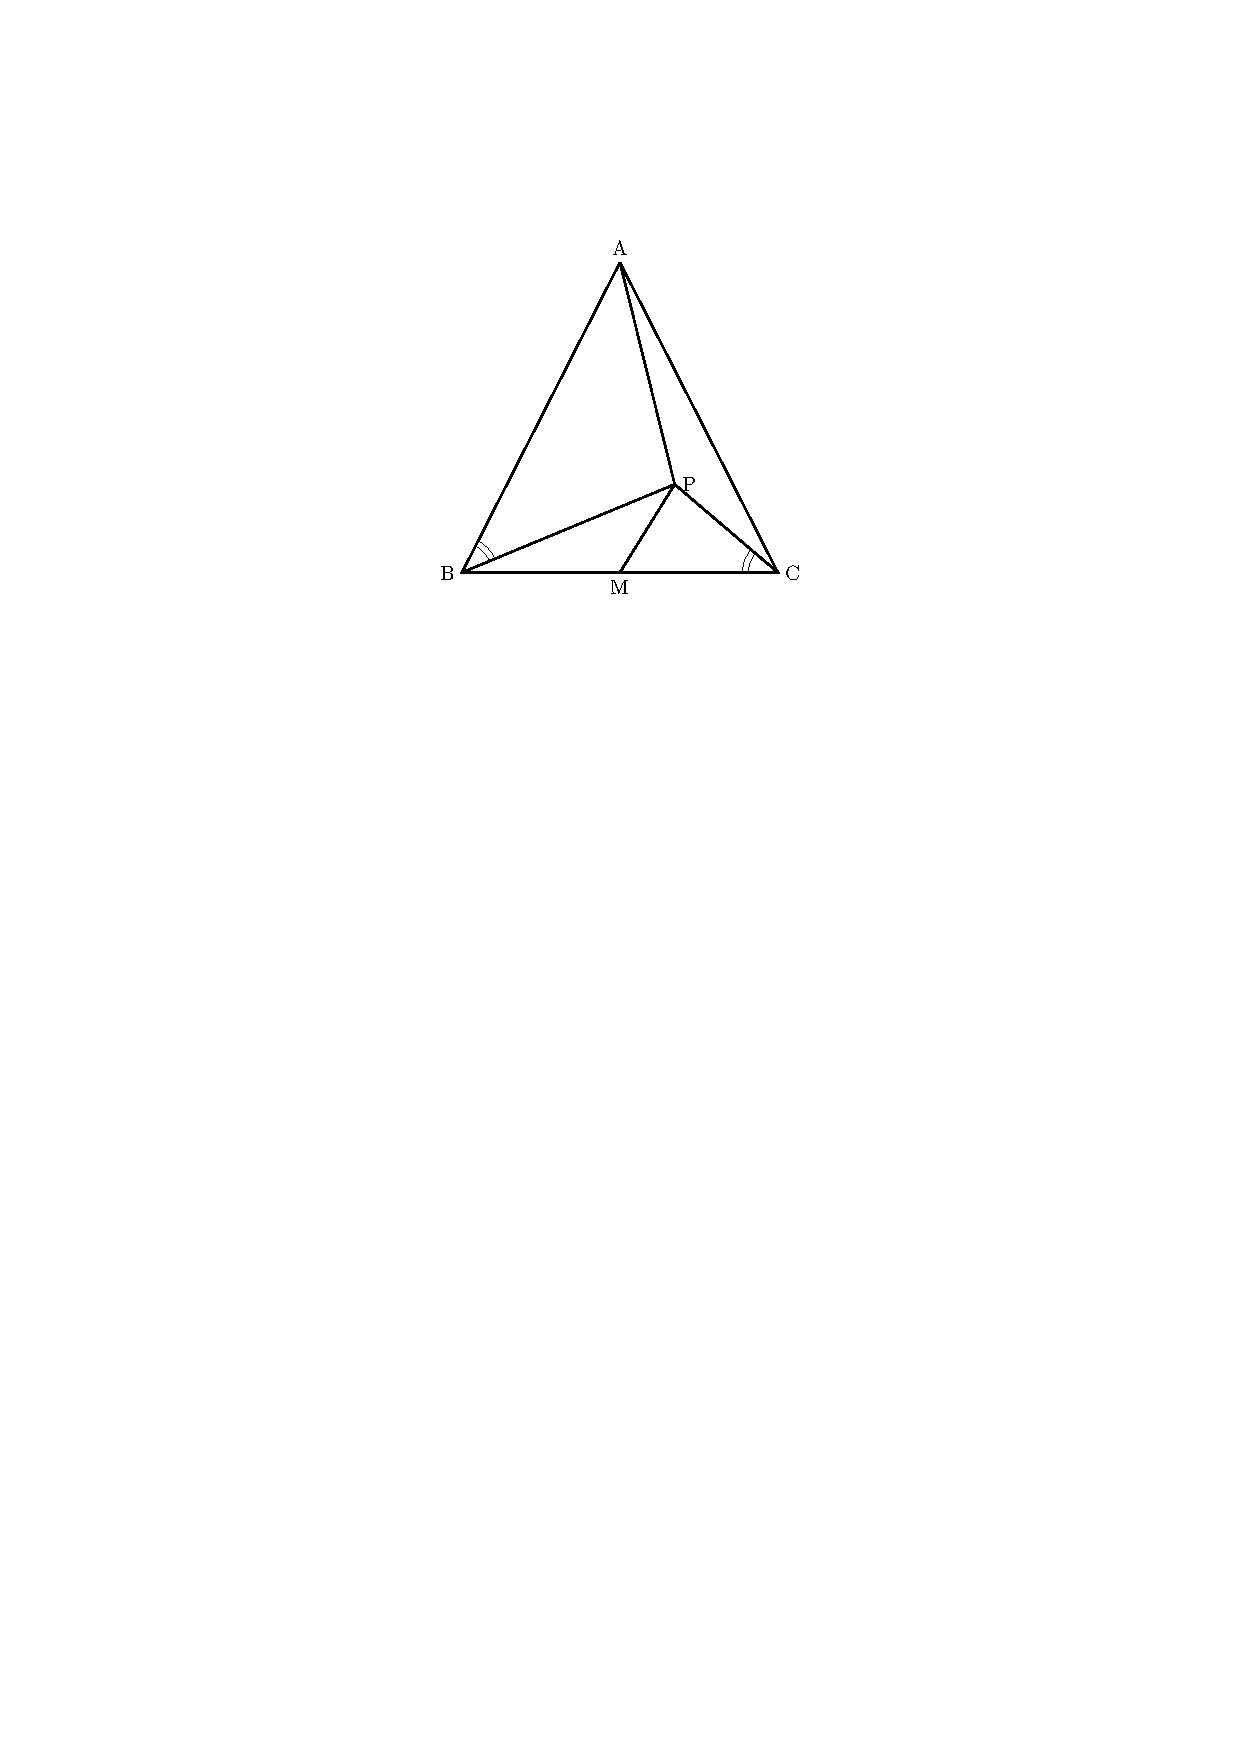
\includegraphics[width=6.0cm]{jizen_5_2_problem.pdf}
\end{figure}

\end{enumerate}


\newpage

\section*{数学オリンピックワークショップ 事前演習問題G ---解答---}

\fbox{G1}

\begin{enumerate}
\item 下図のように正三角形$\rm XYZ$を作ると$\triangle \rm XYZ = 27$になるので,
\begin{eqnarray*}
\triangle {\rm PAB} + \triangle {\rm PCD} + \triangle {\rm PEF} &=& \dfrac{1}{3}\triangle {\rm PXY} + \dfrac{1}{3}\triangle {\rm PYZ} + \dfrac{1}{3}\triangle {\rm PZX} \\
&=& \dfrac{1}{3} \triangle {\rm XYZ}\\
&=& 9
\end{eqnarray*}

\begin{figure}[ht]
  \centering
  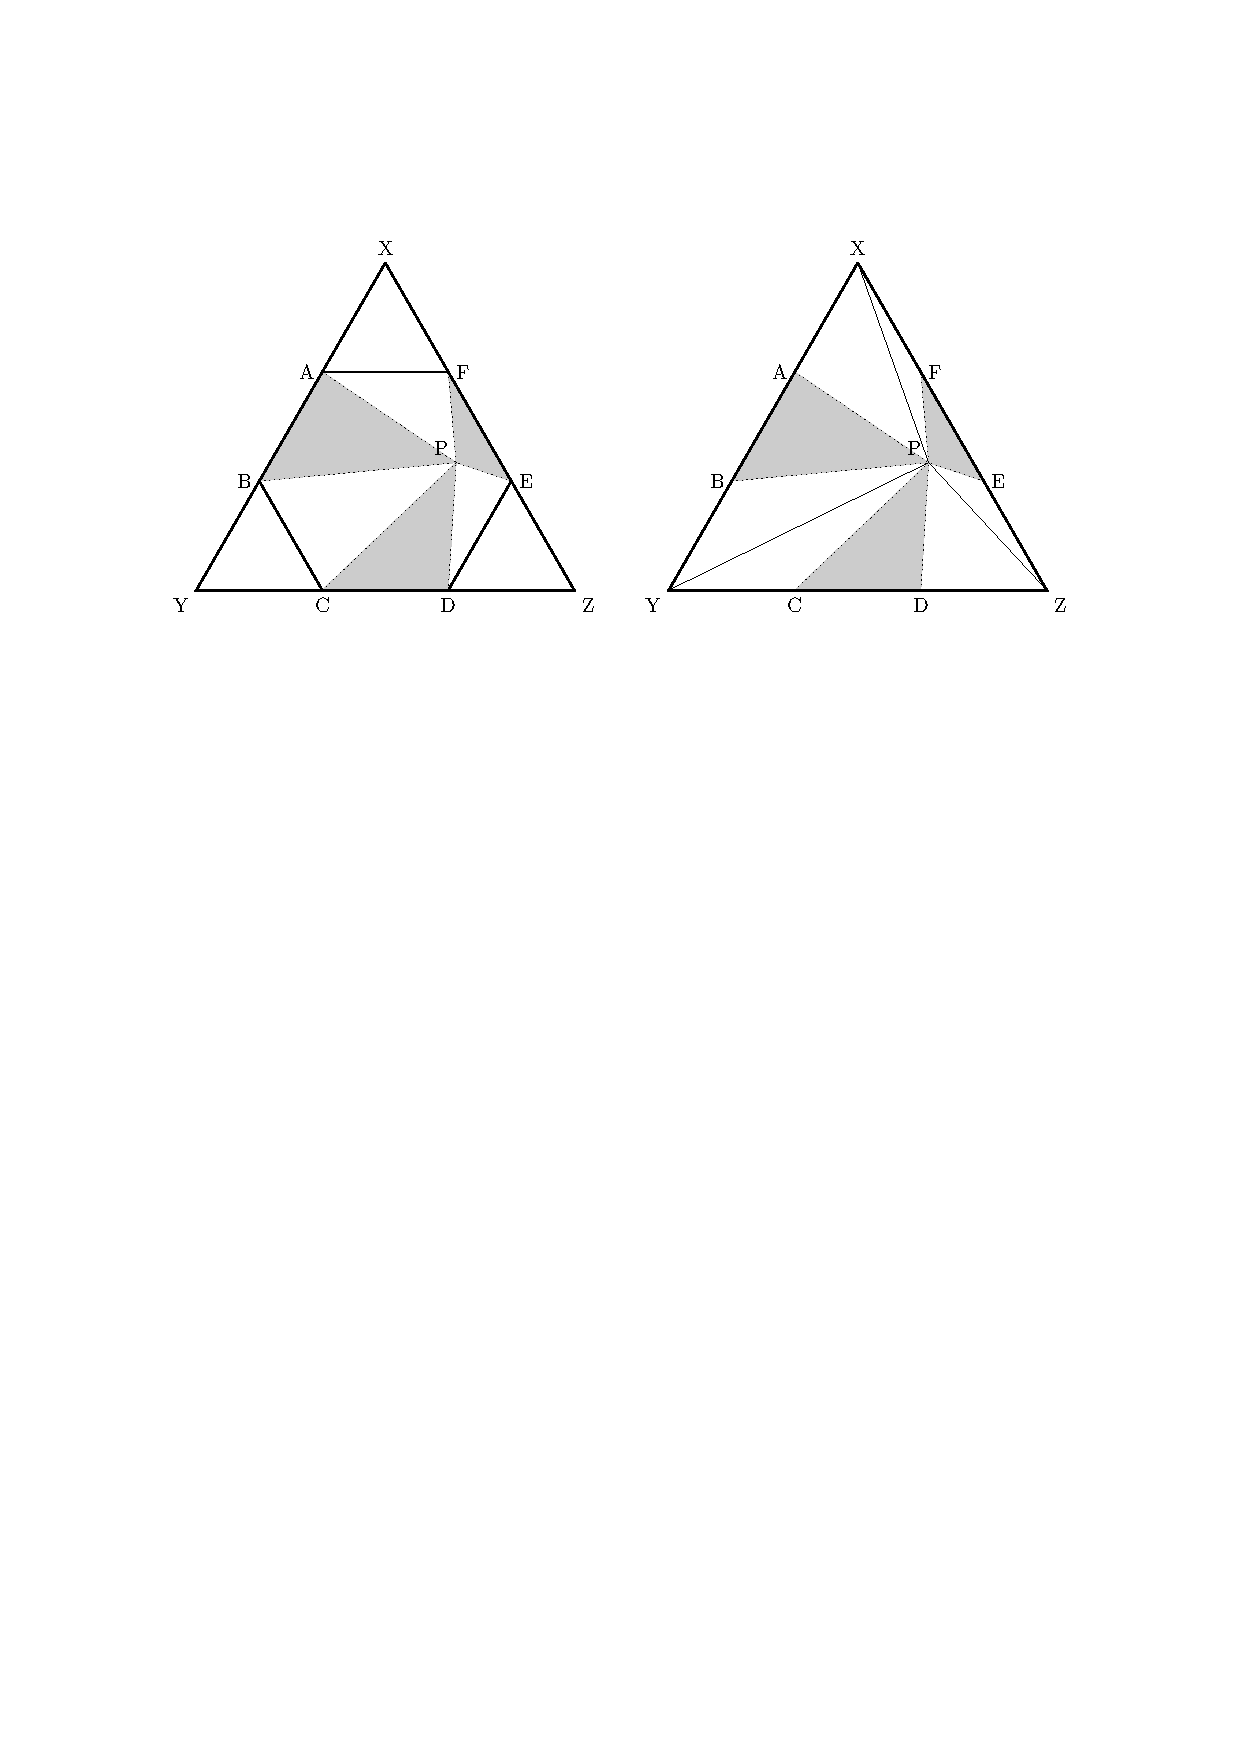
\includegraphics[width=9.0cm]{jizen_1_1_solution.pdf}
\end{figure}

\item 下の図のように$\rm R$をとると,${\rm PR} =x, {\rm QR} = 10-x$とおける。三平方の定理を用いて,
\begin{eqnarray*}
{\rm PQ}^{2} &=& {\rm PR}^{2} + {\rm QR}^{2}\\
&=& x^{2} + (10-x)^{2}\\
&=& 2(x-5)^{2}+50\\
&\ge & 50 \ \ \ \ (等号成立はx=5のとき)
\end{eqnarray*}
ゆえに,$\rm PQ$の最小値は$5\sqrt 2$である。

\begin{figure}[ht]
  \centering
  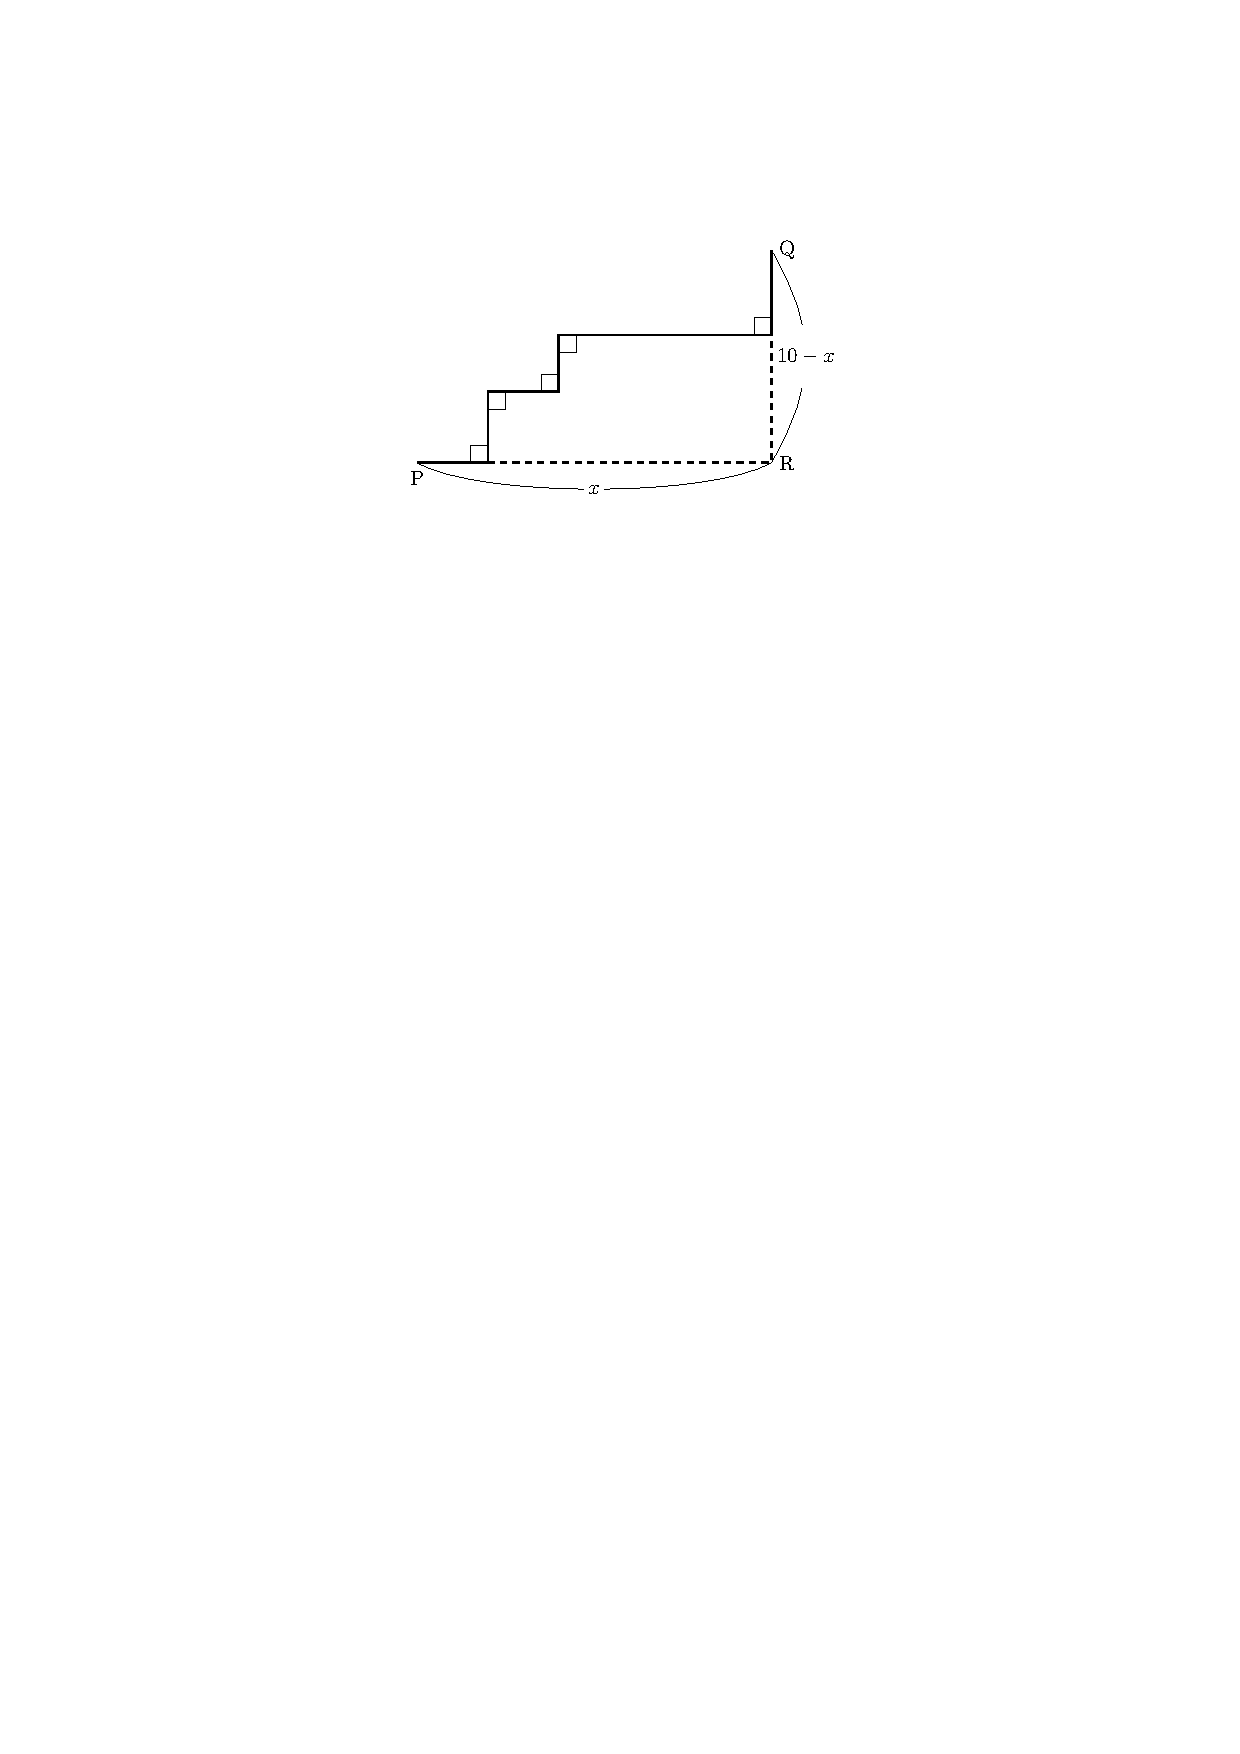
\includegraphics[width=7.0cm]{jizen_1_2_solution.pdf}
\end{figure}

\end{enumerate}

\bigskip

\fbox{G2}

\begin{enumerate}
\item PXと円O,PYと円OのP以外の交点をそれぞれ${\rm X', Y'}$とおくと,直径に関する対称性から${\rm PX}={\rm XX'}, {\rm PY}={\rm YY'}$。よって,中点連結定理から${\rm XY} = \dfrac{{\rm X'Y'}}{2}$。

また簡単な計算から$\angle{\rm Y'PX'}=30^{\circ}$であることがわかる。円周角の定理と合わせて$\triangle {\rm OY'X'}$は正三角形。

ゆえに,${\rm XY} = \dfrac{{\rm X'Y'}}{2} = \dfrac{{\rm OX'}}{2} = \dfrac{4}{2}=2$

\begin{figure}[h]
  \centering
  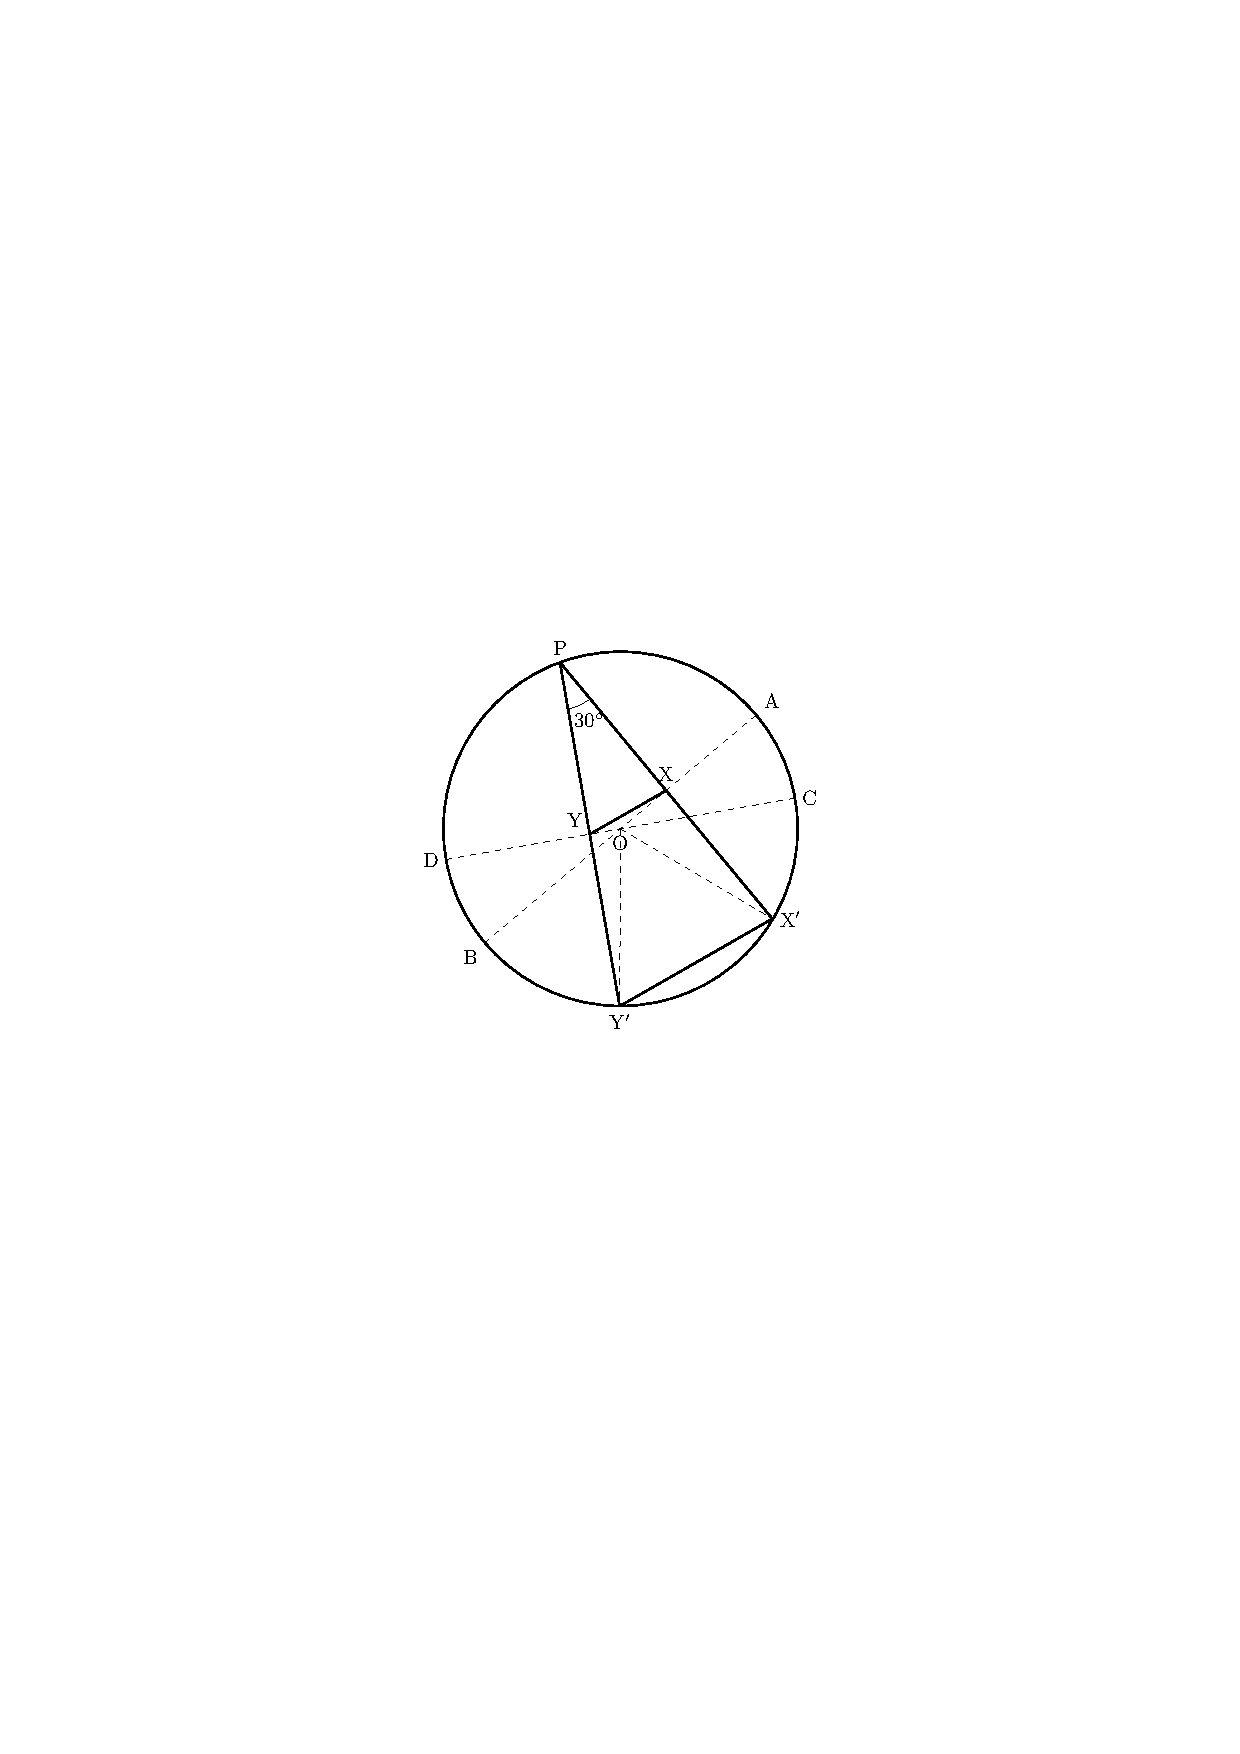
\includegraphics[width=6.0cm]{jizen_2_1_solution.pdf}
\end{figure}

\bigskip

\item $\triangle{\rm ABP}\sim\triangle{\rm EDP}, \triangle{\rm PCD}\sim\triangle{\rm PAF}, \triangle{\rm BCP}\sim\triangle{\rm FEP}$より,
$$\frac{{\rm DE}}{{\rm AB}} = \frac{{\rm PD}}{{\rm PB}}, \ \ \ \frac{{\rm FA}}{{\rm CD}} = \frac{{\rm PF}}{{\rm PD}}, \ \ \ \frac{{\rm BC}}{{\rm EF}} = \frac{{\rm PB}}{{\rm PF}}$$

よって,
$$\frac{{\rm DE}}{{\rm AB}} \cdot \frac{{\rm FA}}{{\rm CD}} \cdot \frac{{\rm BC}}{{\rm EF}} = \frac{{\rm PD}}{{\rm PB}} \cdot \frac{{\rm PF}}{{\rm PD}} \cdot \frac{{\rm PB}}{{\rm PF}} = 1$$

つまり,
$$\rm AB \cdot CD \cdot EF = \rm BC \cdot DE \cdot FA$$

${\rm AB}=3, {\rm BC}=4, {\rm CD}=5, {\rm DE}=6, {\rm EF}=9$を代入して,${\rm FA}=\dfrac{45}{8}$
\begin{figure}[h]
  \centering
  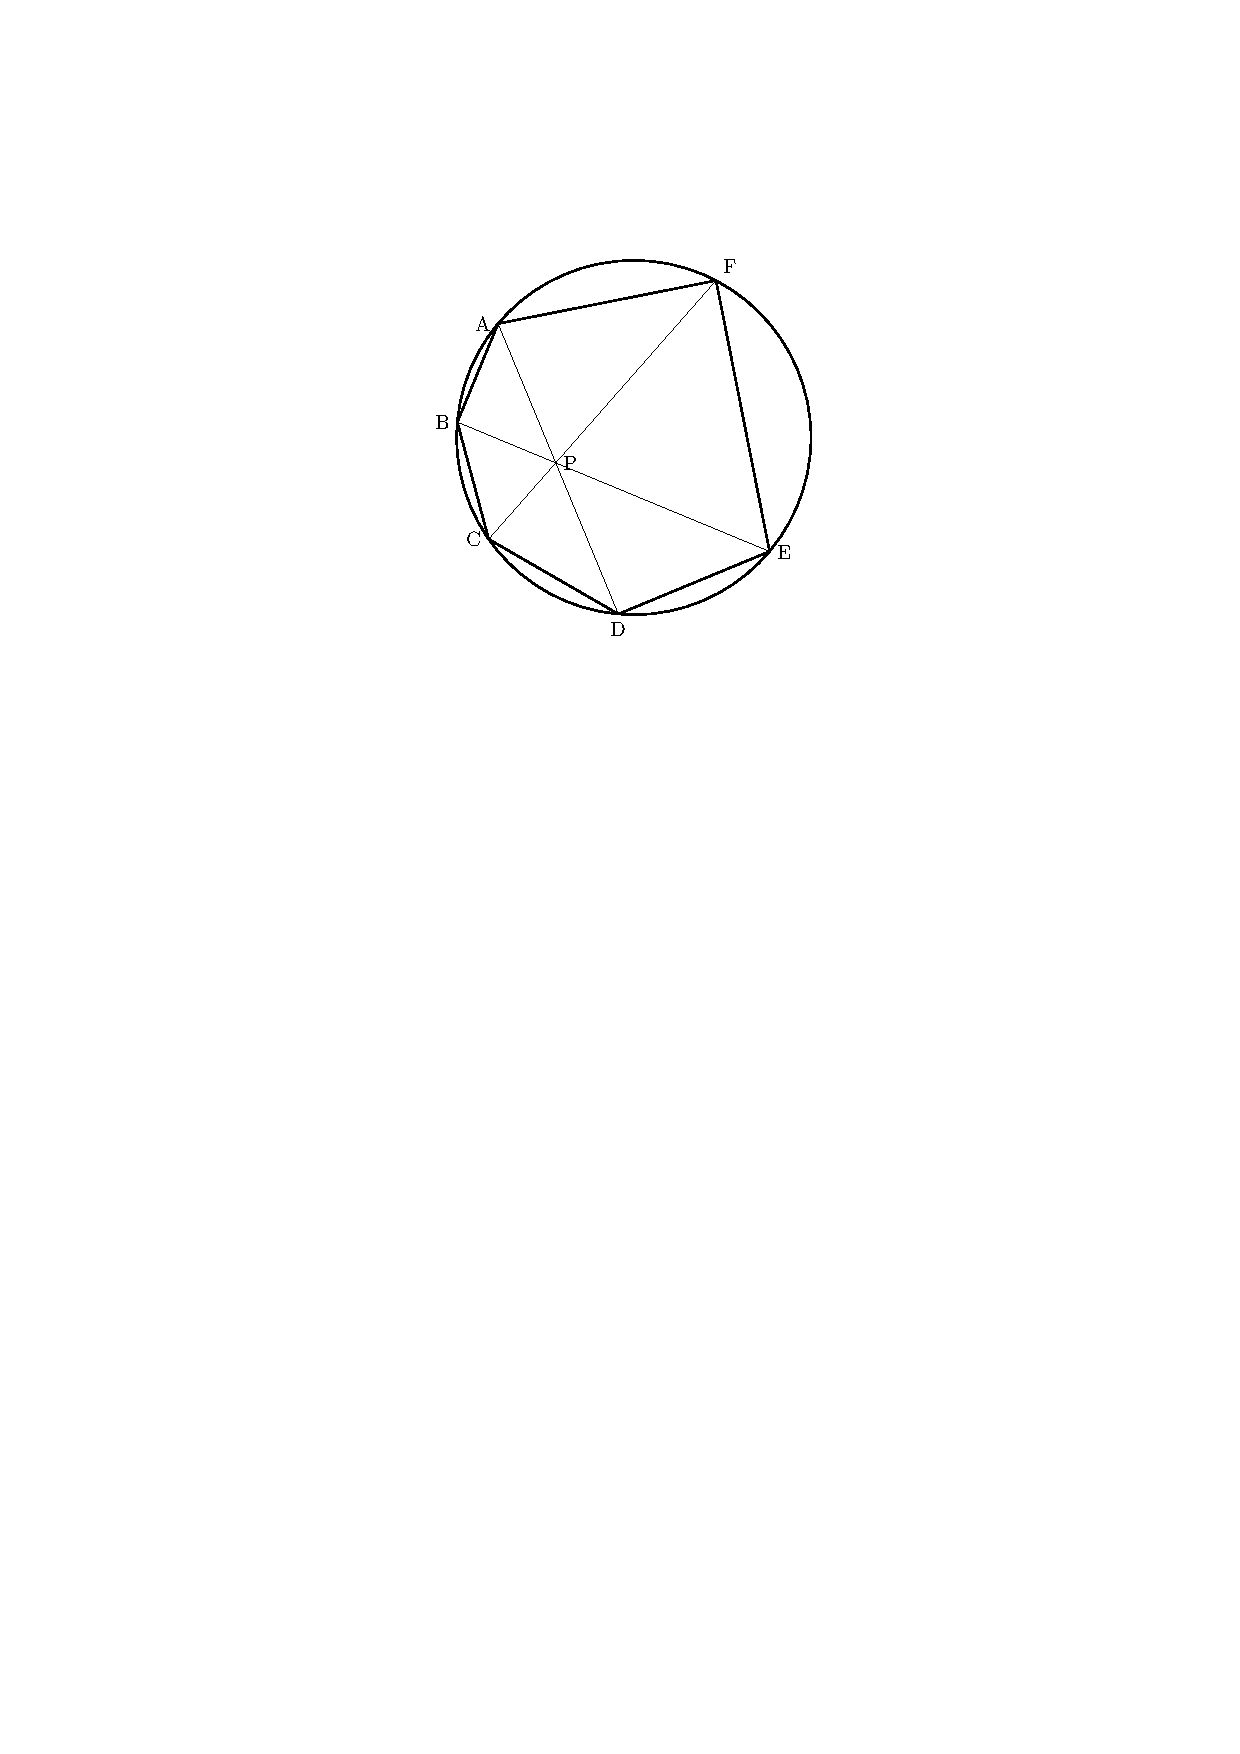
\includegraphics[width=5.0cm]{jizen_2_2_solution.pdf}
\end{figure}



\end{enumerate}

\bigskip

\fbox{G3}

\begin{enumerate}
\item ${\rm PA}=x, {\rm PB}=y, {\rm PC}=z$, $\angle {\rm APB}=90^{\circ}, \angle {\rm BPC}=120^{\circ}$になるように$\rm P, A, B ,C$を定めると,余弦定理および与えられた条件式から${\rm AB}=3, {\rm BC}=5, {\rm CA}=4$。よって,
\begin{eqnarray*}
xy+\dfrac{\sqrt 3}{2}yz+\dfrac{1}{2}zx &=& 2(\triangle{\rm PAB}+\triangle{\rm PBC}+\triangle{\rm PCA})\\
&=&2 \triangle{\rm ABC}\\
&=&3\times 4\\
&=&12
\end{eqnarray*}


\begin{figure}[ht]
  \centering
  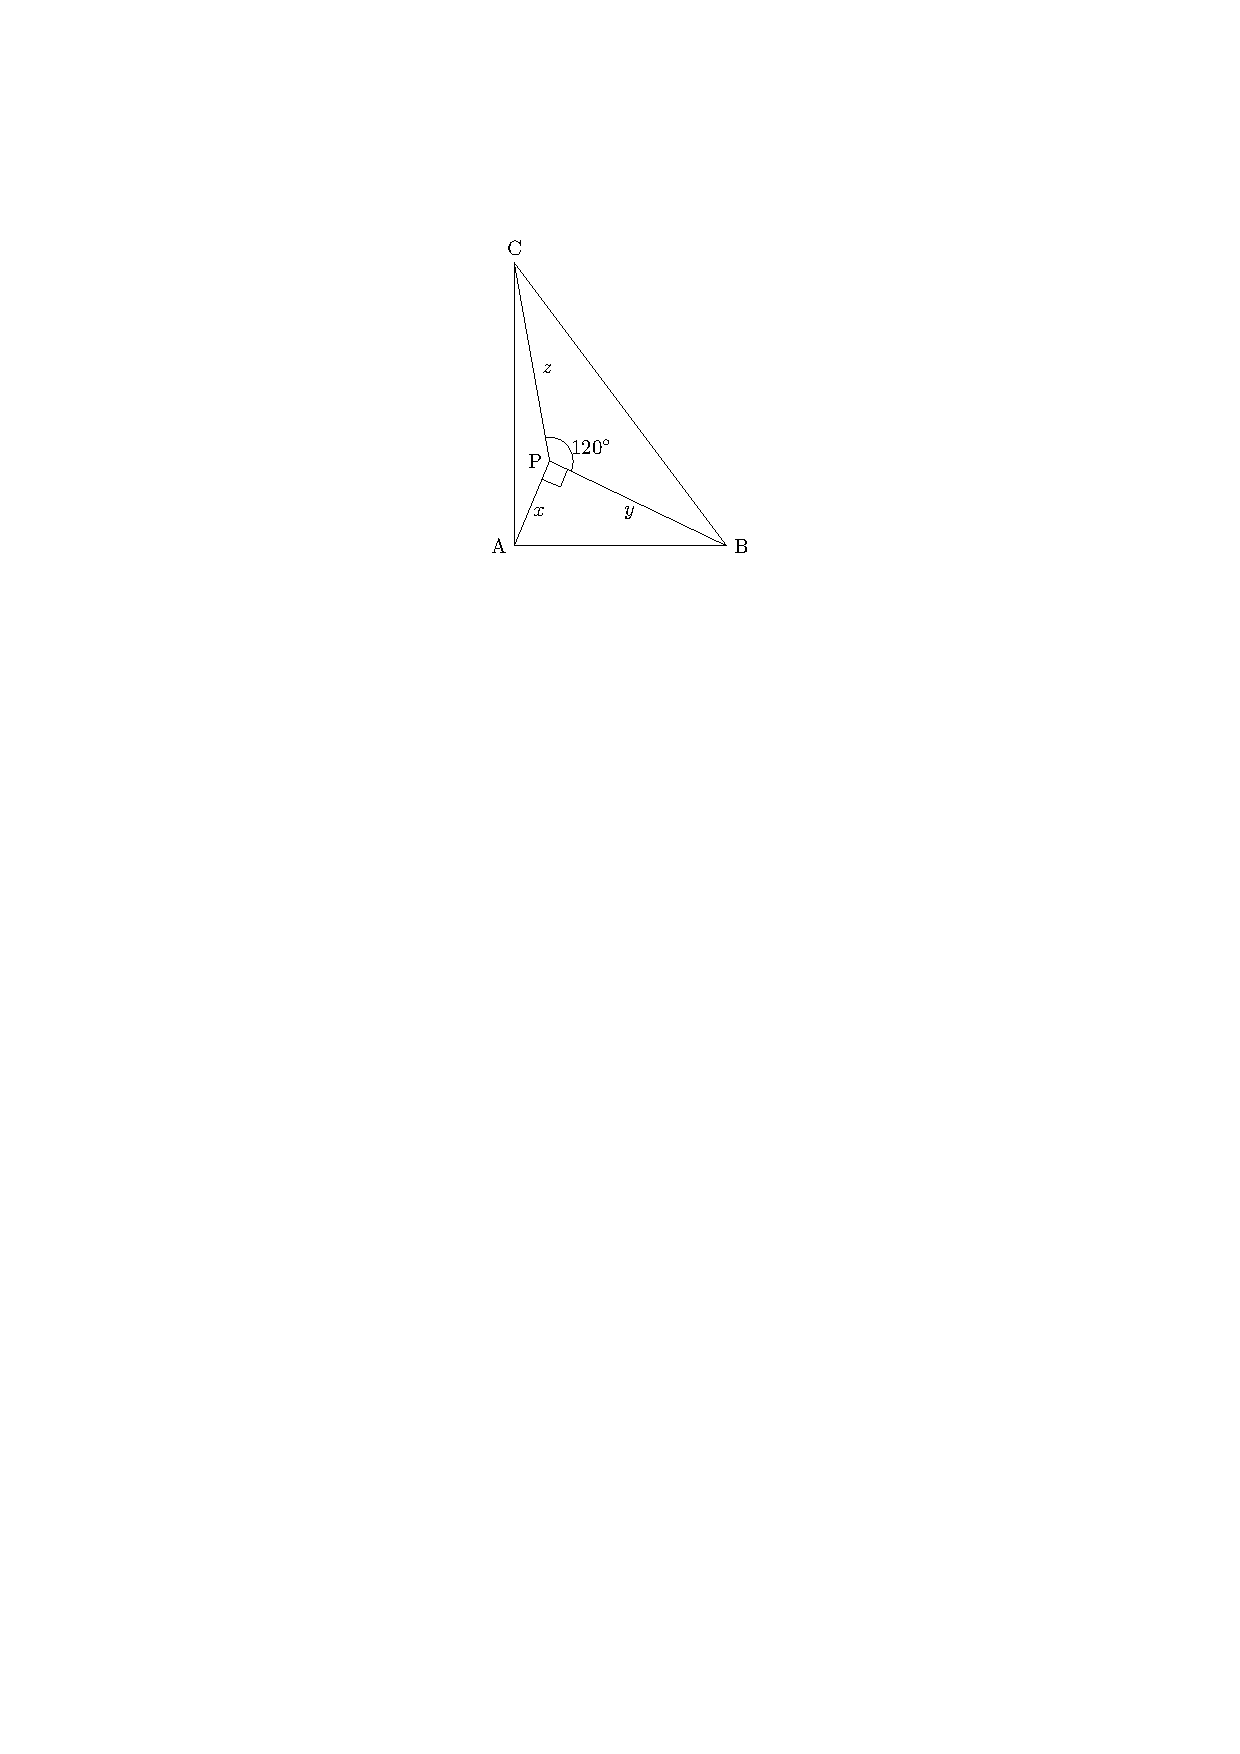
\includegraphics[width=5.0cm]{jizen_3_1_solution.pdf}
\end{figure}


\item 
$\overrightarrow{p}=(a,b)$, $\overrightarrow{q}=(c,d)$, $\overrightarrow{r}=(e,f)$, $\overrightarrow{s}=(g,h)$とおくと,$ac+bd, ce+df, eg+fh, ga+hb, ae+bf, cg+dh$はそれぞれ$\overrightarrow{p}\cdot\overrightarrow{q}, \overrightarrow{q}\cdot\overrightarrow{r}, \overrightarrow{r}\cdot\overrightarrow{s}, \overrightarrow{s}\cdot\overrightarrow{p}, \overrightarrow{p}\cdot\overrightarrow{r}, \overrightarrow{q}\cdot\overrightarrow{s}$の6つの内積と対応する。$\overrightarrow{p}, \overrightarrow{q}, \overrightarrow{r}, \overrightarrow{s}$のどれかが$\overrightarrow{0}$であれば題意は明らか。そうでない場合,$\overrightarrow{p}, \overrightarrow{q}, \overrightarrow{r}, \overrightarrow{s}$の中からそのなす角が$90^{\circ}$以下である2つのベクトルがとれる。その2つのベクトルの内積は0以上。



\begin{figure}[ht]
  \centering
  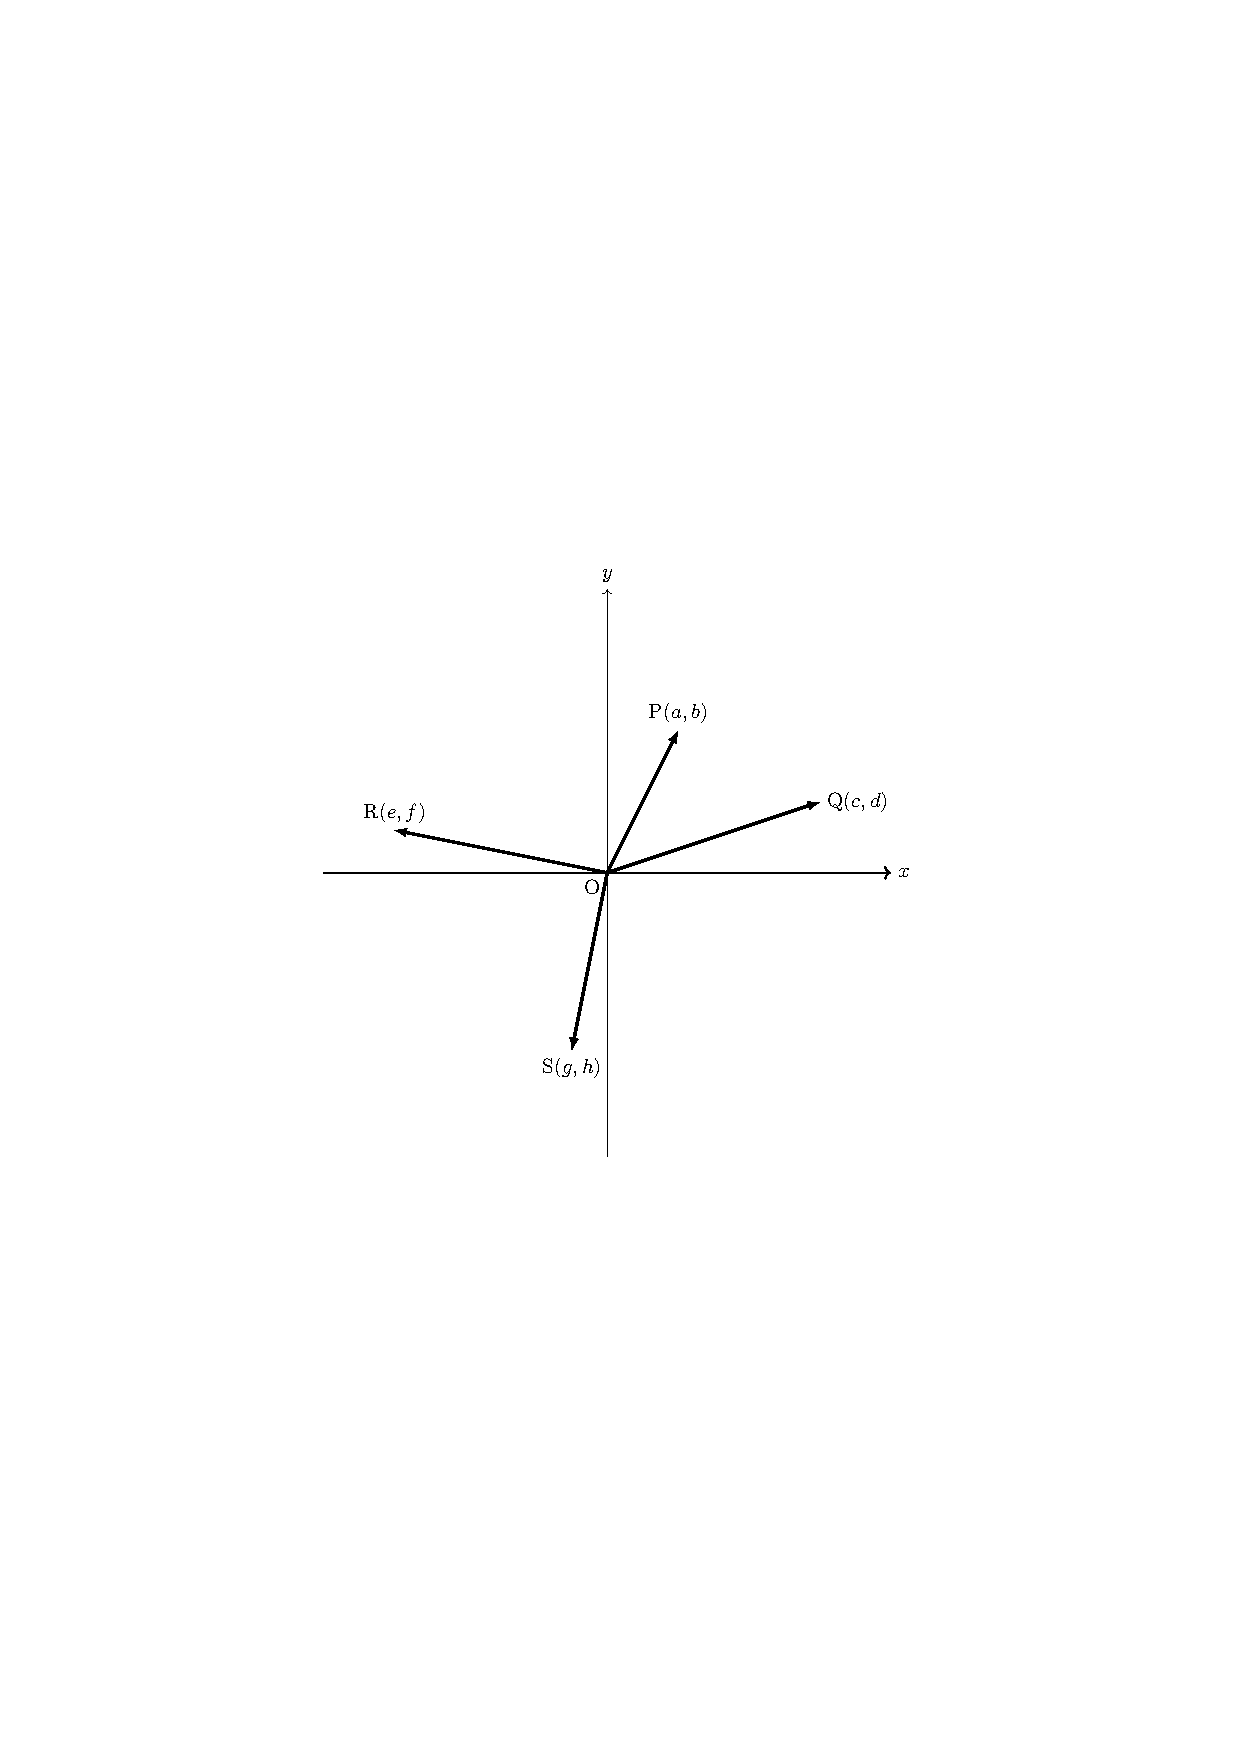
\includegraphics[width=6.0cm]{jizen_3_2_solution.pdf}
\end{figure}


\end{enumerate}

\bigskip

\fbox{G4}

\begin{enumerate}
\item ${\rm OA}={\rm OB}={\rm OC}={\rm OD}=a, \ {\rm OP}=p, {\rm OQ}=q, {\rm OR}=r, {\rm OS}=s, \ ({\rm O-ABCD}の体積)=V$とおくと,${\rm O-PQRS}$の体積を2通りで表して,
\begin{eqnarray*}
({\rm O-PQRS}の体積) &=& (三角錐{\rm O-PQR}の体積)+(三角錐{\rm O-RSP}の体積) \\
                     &=& \frac{V}{2}\cdot\frac{p}{a}\cdot\frac{q}{a}\cdot\frac{r}{a}+\frac{V}{2}\cdot\frac{r}{a}\cdot\frac{s}{a}\cdot\frac{p}{a}\\[8pt]
({\rm O-PQRS}の体積) &=& (三角錐{\rm O-QRS}の体積)+(三角錐{\rm O-SPQ}の体積) \\
                     &=& \frac{V}{2}\cdot\frac{q}{a}\cdot\frac{r}{a}\cdot\frac{s}{a}+\frac{V}{2}\cdot\frac{s}{a}\cdot\frac{p}{a}\cdot\frac{q}{a}
\end{eqnarray*}
よって,
\begin{eqnarray*}
&&pqr+rsp=qrs+spq \\[5pt]
&\therefore& \frac{1}{p}+\frac{1}{r}=\frac{1}{q}+\frac{1}{s}
\end{eqnarray*}
今回は$p=2,q=4,r=3$なので,$s=\dfrac{12}{7}$とわかる。


\bigskip

\item ${\rm OA}={\rm OB}={\rm OC}={\rm OD}=a, \ {\rm OP}=p, {\rm OQ}=q, {\rm OR}=r, {\rm OS}=s$とおくと,直角三角形の相似およびメネラウスの定理から,

\begin{align*}
&&&&&{\rm CZ} = {\rm BY}\cdot\frac{{\rm XC}}{{\rm BX}}  &\Leftrightarrow& \ \ \frac{1}{{\rm CZ}} = \frac{1}{{\rm BY}} \cdot \frac{{\rm BX}}{{\rm XC}} &&&&\\[7pt]
&&&&&\frac{{\rm BY}}{{\rm YA}} \cdot \frac{{\rm AP}}{{\rm PO}} \cdot \frac{{\rm OQ}}{{\rm QB}}=1 &\Leftrightarrow& \ \ 1+\frac{\sqrt 2 a}{{\rm BY}} = \frac{a-p}{p}\cdot\frac{q}{a-q} &&&&\\[7pt]
&&&&&\frac{{\rm XC}}{{\rm BX}} \cdot \frac{{\rm RO}}{{\rm CR}} \cdot \frac{{\rm QB}}{{\rm OQ}}=1 &\Leftrightarrow& \ \ \frac{{\rm BX}}{{\rm XC}} = \frac{r}{a-r}\cdot\frac{a-q}{q} &&&&\\[7pt]
&&&&&\frac{{\rm ZD}}{{\rm CZ}} \cdot \frac{{\rm SO}}{{\rm DS}} \cdot \frac{{\rm RC}}{{\rm OR}}=1 &\Leftrightarrow& \ \ 1+\frac{\sqrt 2 a}{{\rm CZ}} = \frac{a-s}{s}\cdot\frac{r}{a-r} &&&&\\[7pt]
\end{align*}

\begin{figure}[ht]
  \centering
  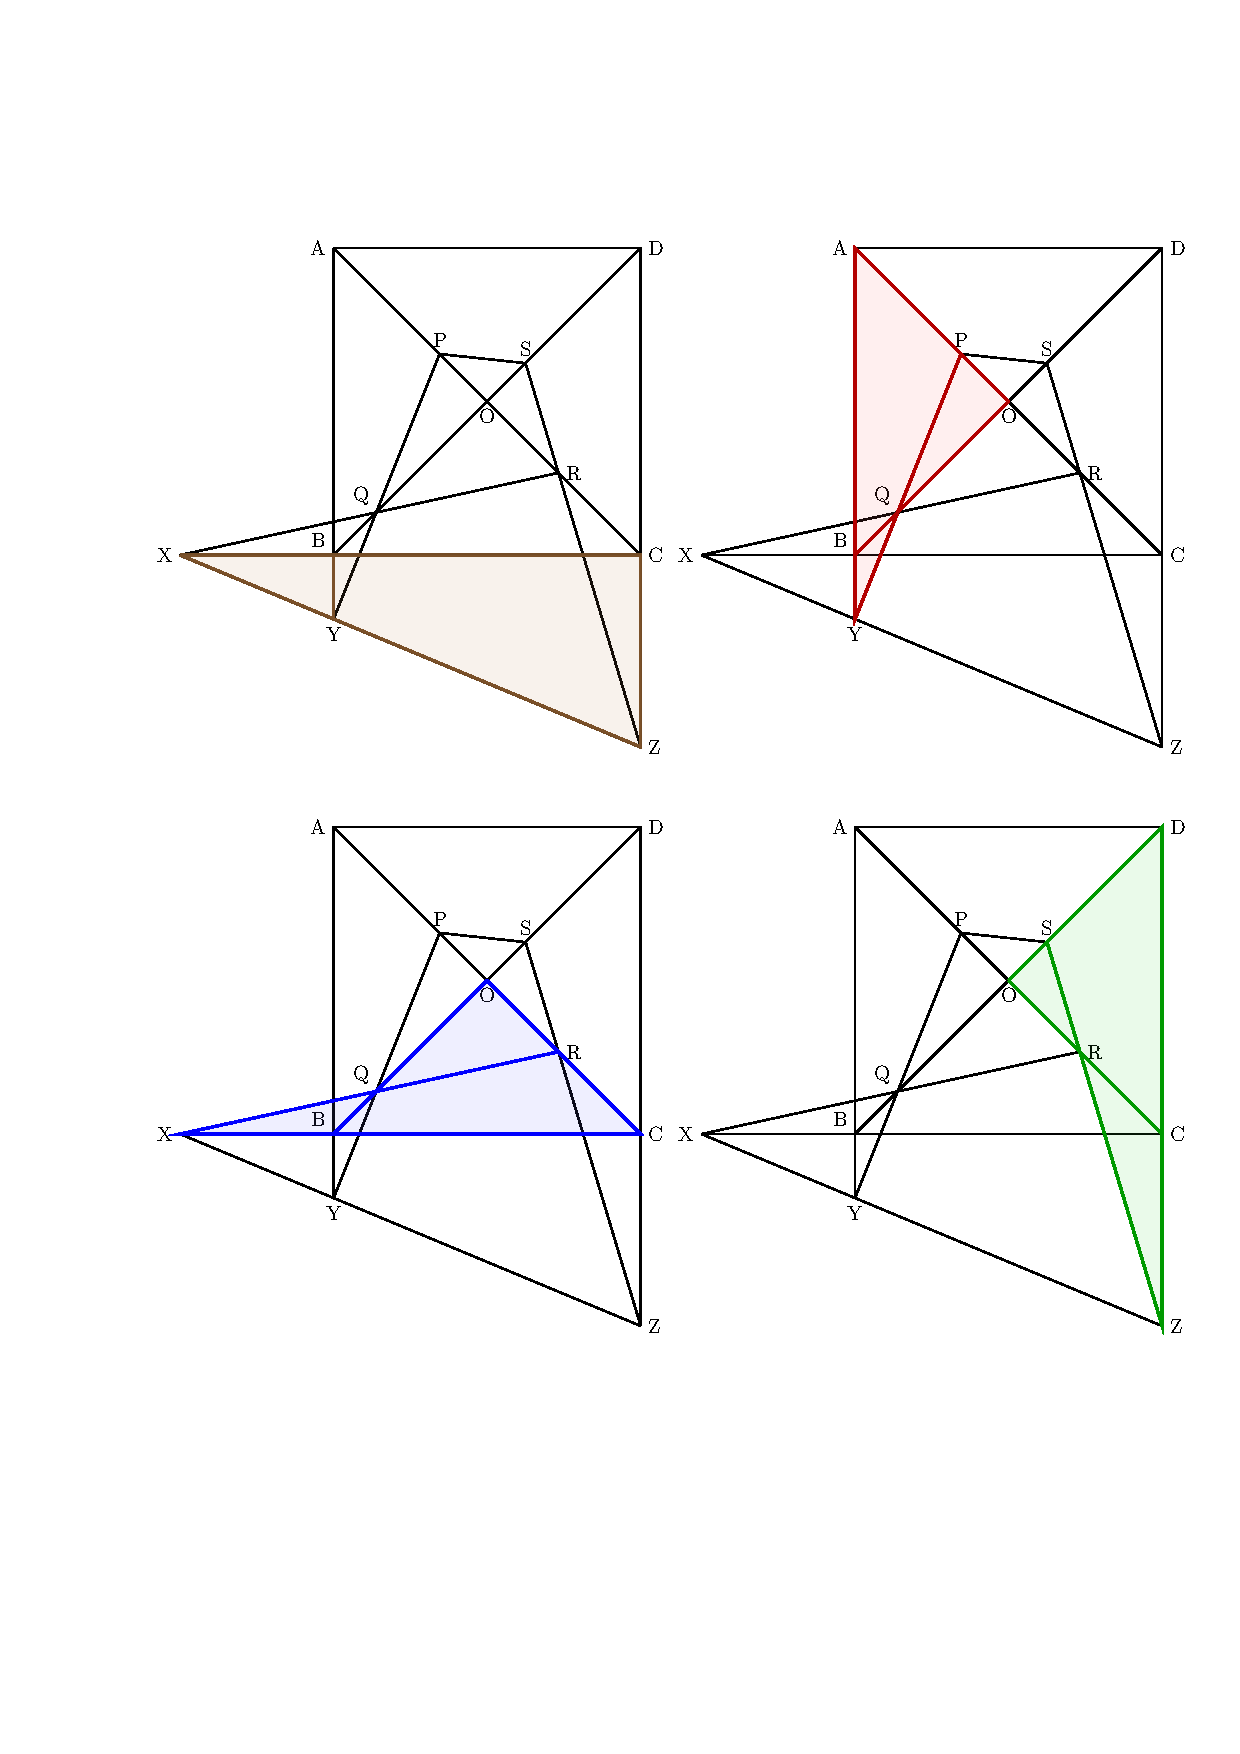
\includegraphics[width=10.0cm]{jizen_4_2_solution.pdf}
\end{figure}

これらを用いて,
\begin{eqnarray*}
\frac{a-s}{s}\cdot\frac{r}{a-r} &=& 1+\frac{\sqrt 2 a}{{\rm CZ}} \\
&=& 1+\frac{\sqrt 2 a}{{\rm BY}} \cdot \frac{{\rm BX}}{{\rm XC}} \\
&=& 1+ \left(\frac{a-p}{p}\cdot\frac{q}{a-q}-1\right)\cdot \frac{r}{a-r}\cdot\frac{a-q}{q}
\end{eqnarray*}

両辺$\dfrac{r}{a-r}$で割って,
\begin{eqnarray*}
&&\frac{a-s}{s} = \frac{a-r}{r}+ \left(\frac{a-p}{p}\cdot\frac{q}{a-q}-1\right)\cdot\frac{a-q}{q} \\
&\Leftrightarrow& \frac{a-s}{s} + \frac{a-q}{q} = \frac{a-r}{r} + \frac{a-p}{p}\\
&\Leftrightarrow& \frac{1}{p}+\frac{1}{r} = \frac{1}{q}+\frac{1}{s}
\end{eqnarray*}

今回は$p=2,q=4,r=3$なので,$s=\dfrac{12}{7}$とわかる。

\bigskip

(\underline{別解})

次の図をよ〜く睨んでいると(1)と(2)が等価であることがわかる。(この図を上から眺めてみよう)
\begin{figure}[ht]
  \centering
  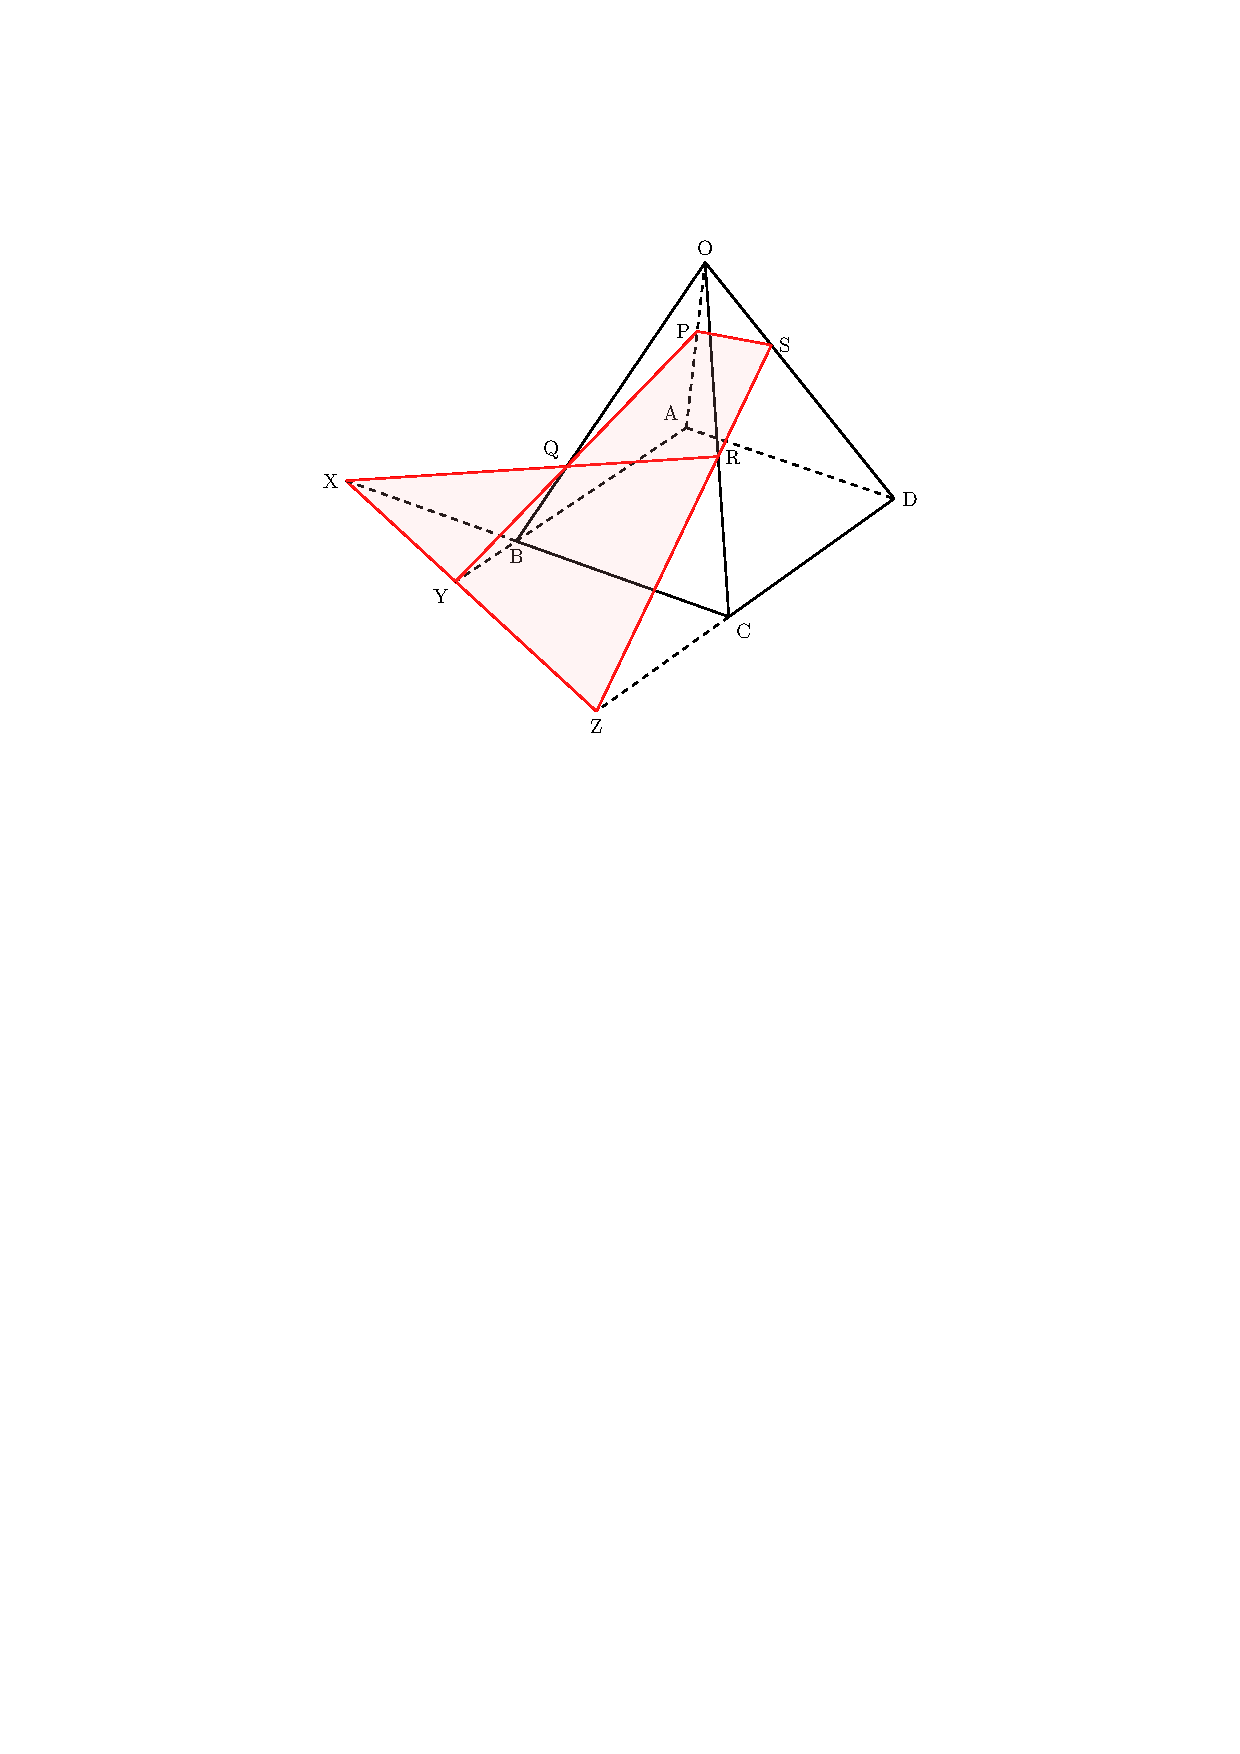
\includegraphics[width=10.0cm]{jizen_4_2_anothersolution.pdf}
\end{figure}


\end{enumerate}

\bigskip

\fbox{G5}

\begin{enumerate}
\item $\triangle{\rm ABC}$の外接円の中心をO,Dを中心としてBを通る円とAB, ACの交点をそれぞれP, Q とすると,
\begin{eqnarray*}
\angle{\rm PBQ} &=& \angle{\rm BAQ} + \angle{\rm BQA}\\
&=& \frac{1}{2} (\angle{\rm BOC} + \angle{\rm BDC}) \ \ \ \ (\because \ 円周角の定理)\\
&=& \frac{1}{2} (360^{\circ}- \angle{\rm OBD} + \angle{\rm OCD}) \\
&=& \frac{1}{2} (360^{\circ}- 90^{\circ}- 90^{\circ}) \\
&=& 90^{\circ}
\end{eqnarray*}
よってQPは円Dの直径であり,DはQPの中点となる。$\triangle{\rm ABC} \sim \triangle{\rm AQP}$という相似において,MはBCの中点,DはQPの中点であることからMとDが対応していることがわかる。ゆえに,$\angle{\rm BAM} = \angle{\rm QAD}$ 。

\begin{figure}[h]
  \centering
  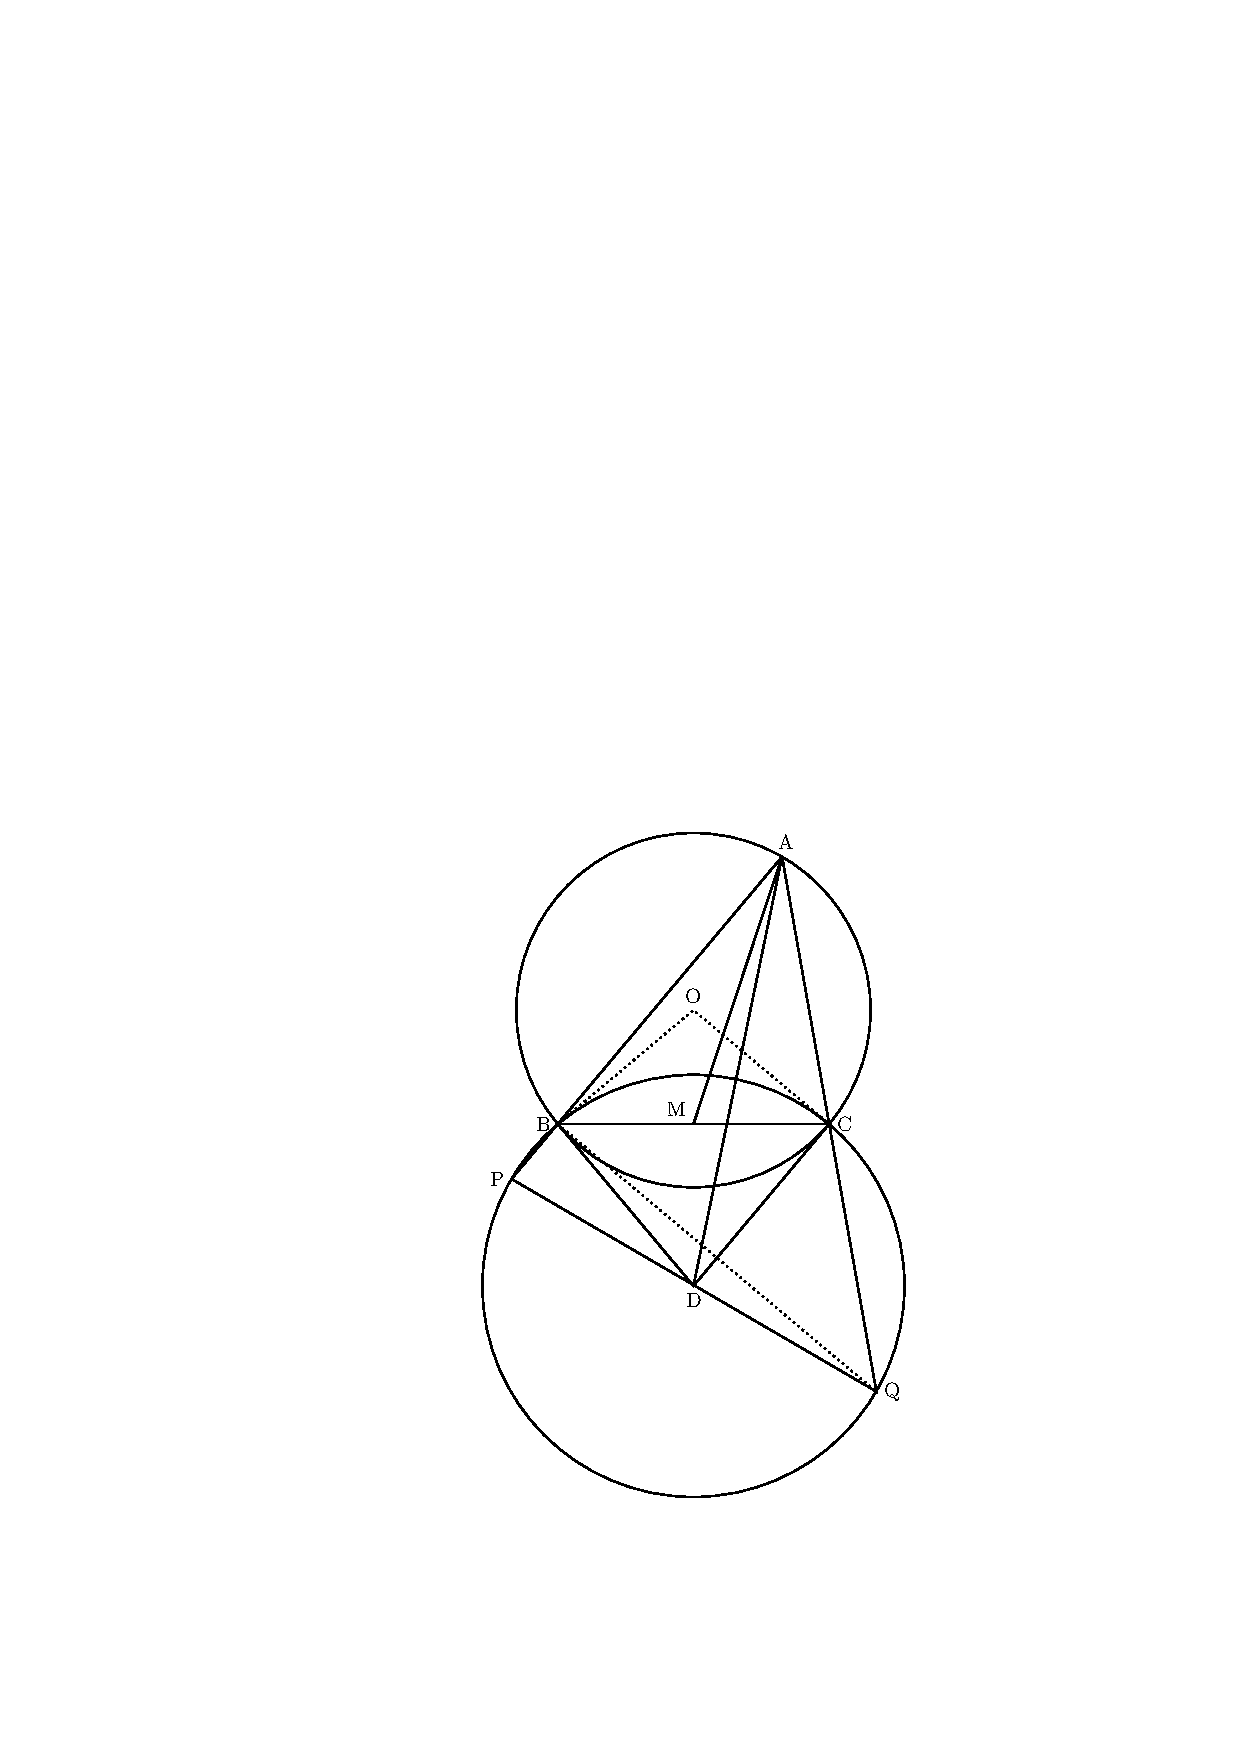
\includegraphics[width=5cm]{jizen_5_1_solution.pdf}
\end{figure}


\item 

$\rm AB=AC$より,$\angle{\rm ABC} = \angle{\rm ACB}$。$\angle{\rm PBA} = \angle{\rm PCB}$と合わせて$\angle{\rm PBC} = \angle{\rm PCA}$。ゆえに接弦定理の逆から,ABとACは$\triangle{\rm PBC}$の外接円の接線であることが分かる。APとその外接円の交点をQとすると,(1)と同様に$\angle{\rm PQC} = \angle{\rm BQM}$。また,$\angle{\rm BQP} = \angle{\rm MQC}$。円周角の定理より$\angle{\rm BPQ} = \angle{\rm MCQ}$であることと合わせて,$\triangle{\rm QPB}\sim \triangle{\rm QCM}$。よって,
\begin{eqnarray*}
&& \frac{{\rm QM}}{{\rm QB}} = \frac{{\rm MC}}{{\rm BP}}\\
&\therefore& \frac{{\rm QM}}{{\rm QB}} = \frac{{\rm BM}}{{\rm BP}}
\end{eqnarray*}
$\angle{\rm BQM}=\angle{\rm PQC} = \angle{\rm PBM}$と合わせて,$\triangle{\rm QBM}\sim \triangle{\rm BPM}$。ゆえに,
$$\angle{\rm APC} + \angle{\rm BPM}=\angle{\rm APC} + \angle{\rm QBM} =\angle{\rm APC} + \angle{\rm QPC} = 180^{\circ}$$


\begin{figure}[h]
  \centering
  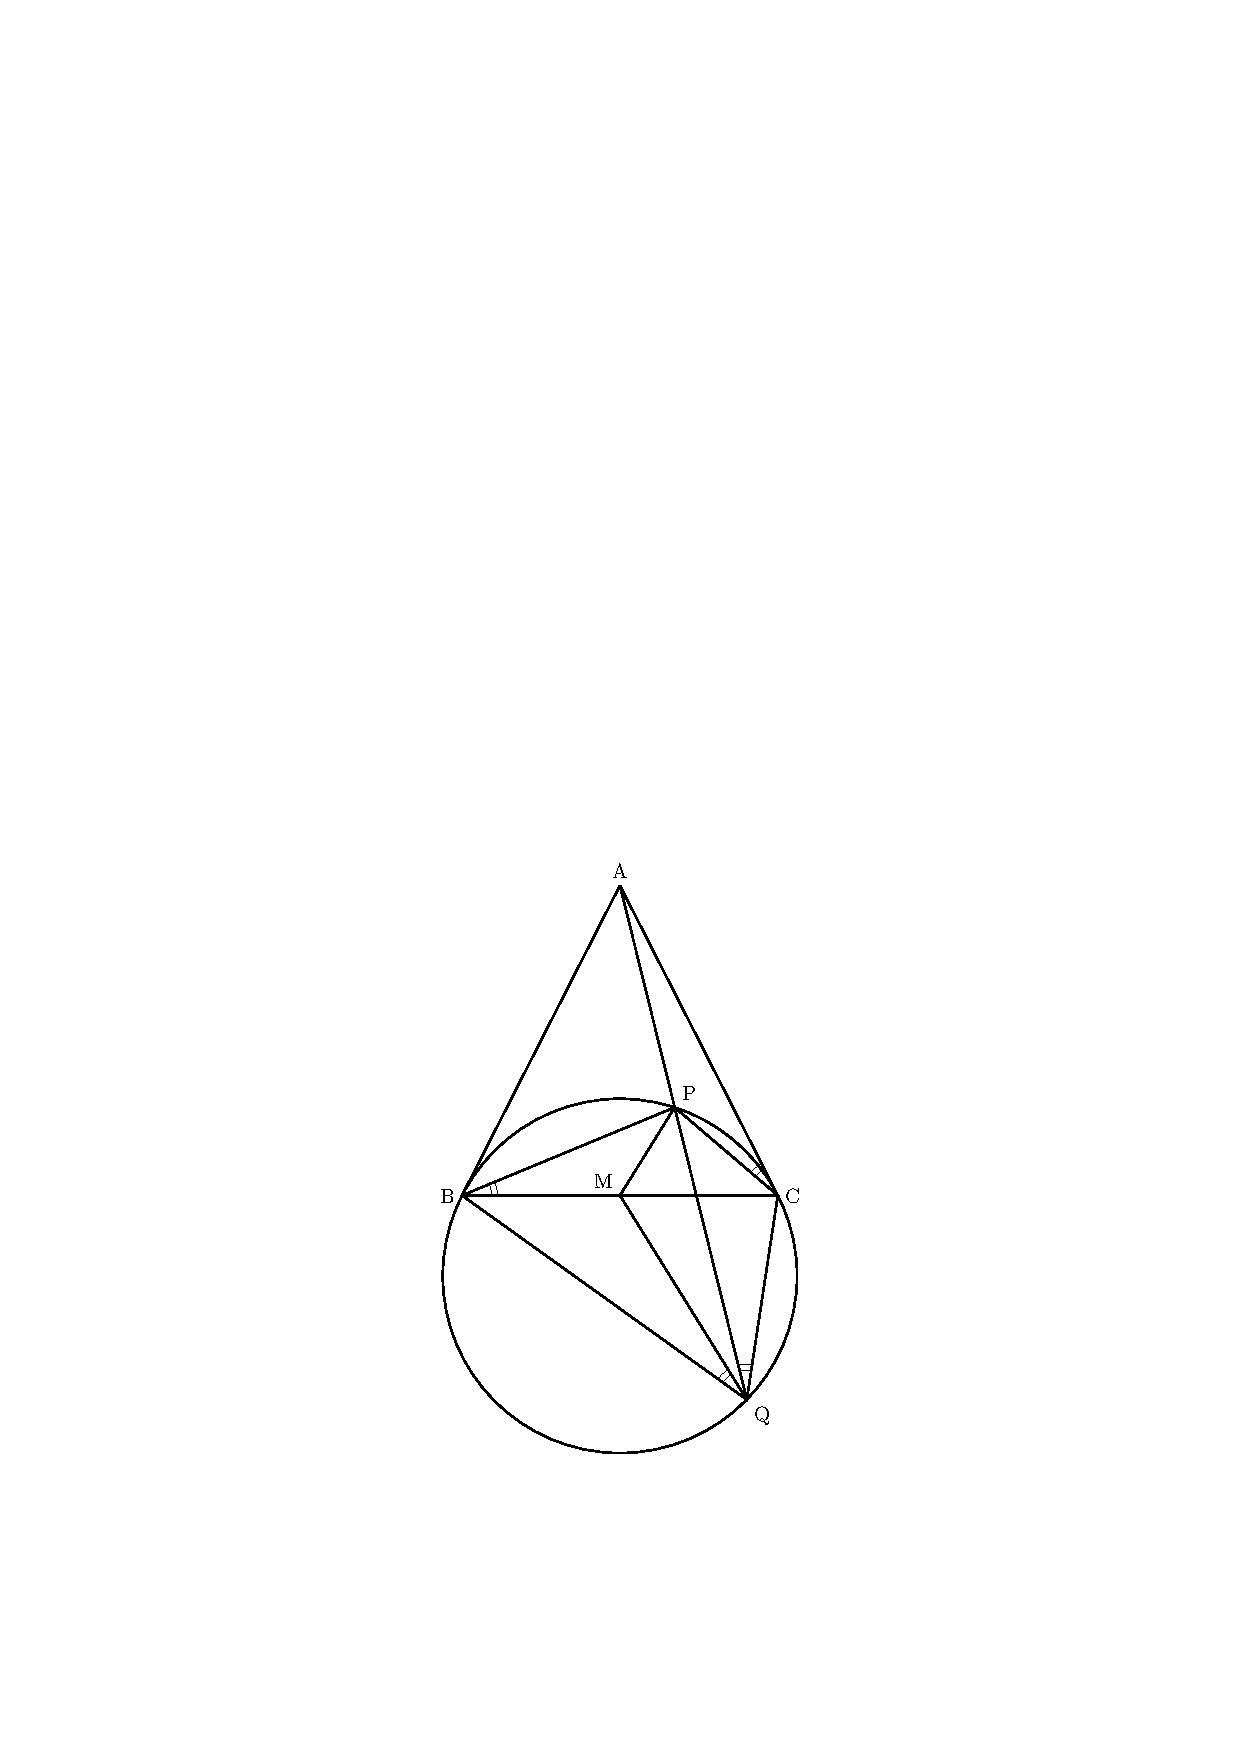
\includegraphics[width=4.8cm]{jizen_5_2_solution.pdf}
\end{figure}

\end{enumerate}













\newpage

\section*{数学オリンピックワークショップ 当日問題G}

\fbox{G6} (基礎)

半径6,中心角$90^{\circ}$の扇形OABの弧AB上に$\angle {\rm AOP} = \angle {\rm BOQ}$となるように点P, Qをとる。点Xが線分OB上を動くとき,$\rm PX+QX$の最小値を求めよ。

\begin{figure}[ht]
  \centering
  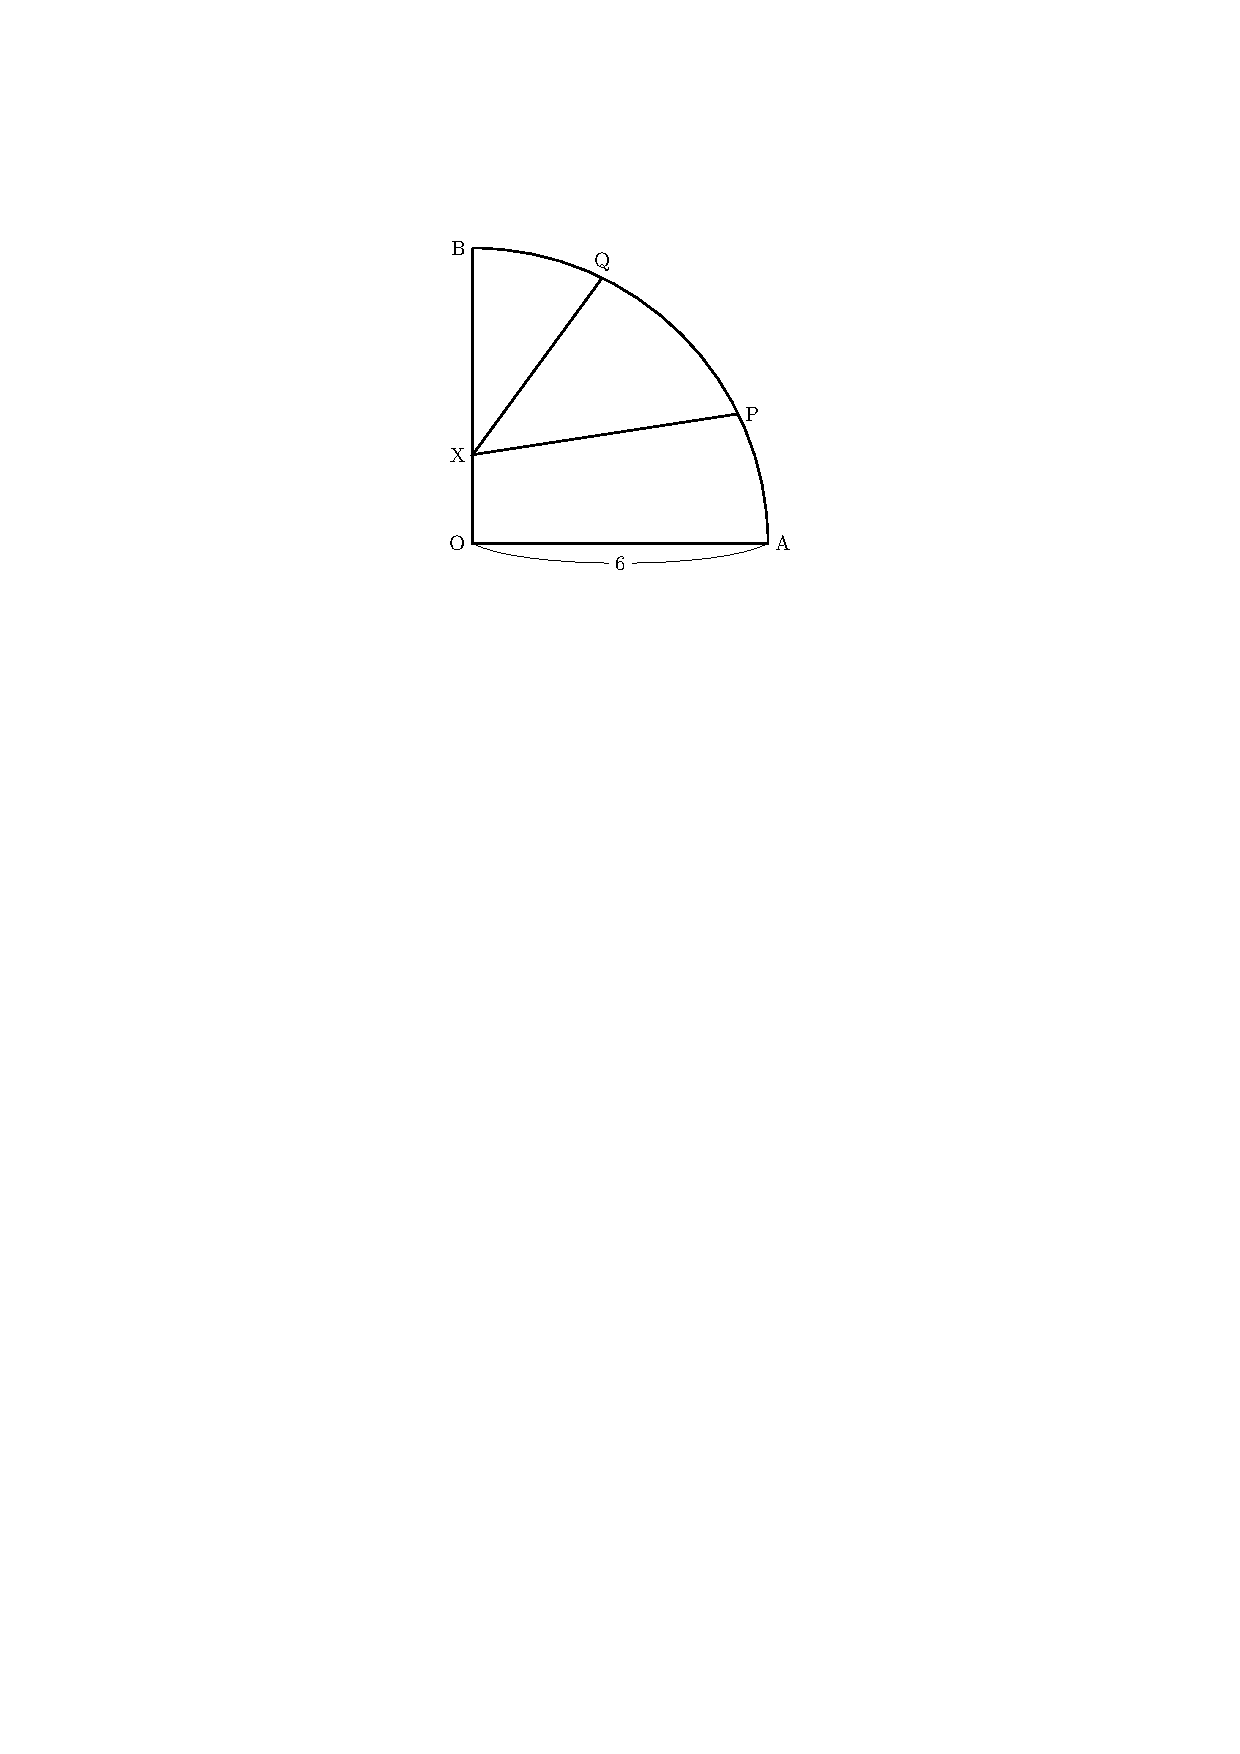
\includegraphics[width=6.0cm]{toujitsu_6_problem.pdf}
\end{figure}

\fbox{G7} (応用)

2つの円が平面上で2点A, Bで交わっている。この2円の共通接線を$l$とし,$l$と2円はそれぞれ点P, Qで接しているものとする。また$\triangle {\rm PAQ}$の外接円のP, Qにおける接線の交点をSとする。$\rm B'$を$l$に関するBの対称点とするとき,$\rm A, B', S$は同一直線上にあることを示せ。

\begin{figure}[ht]
  \centering
  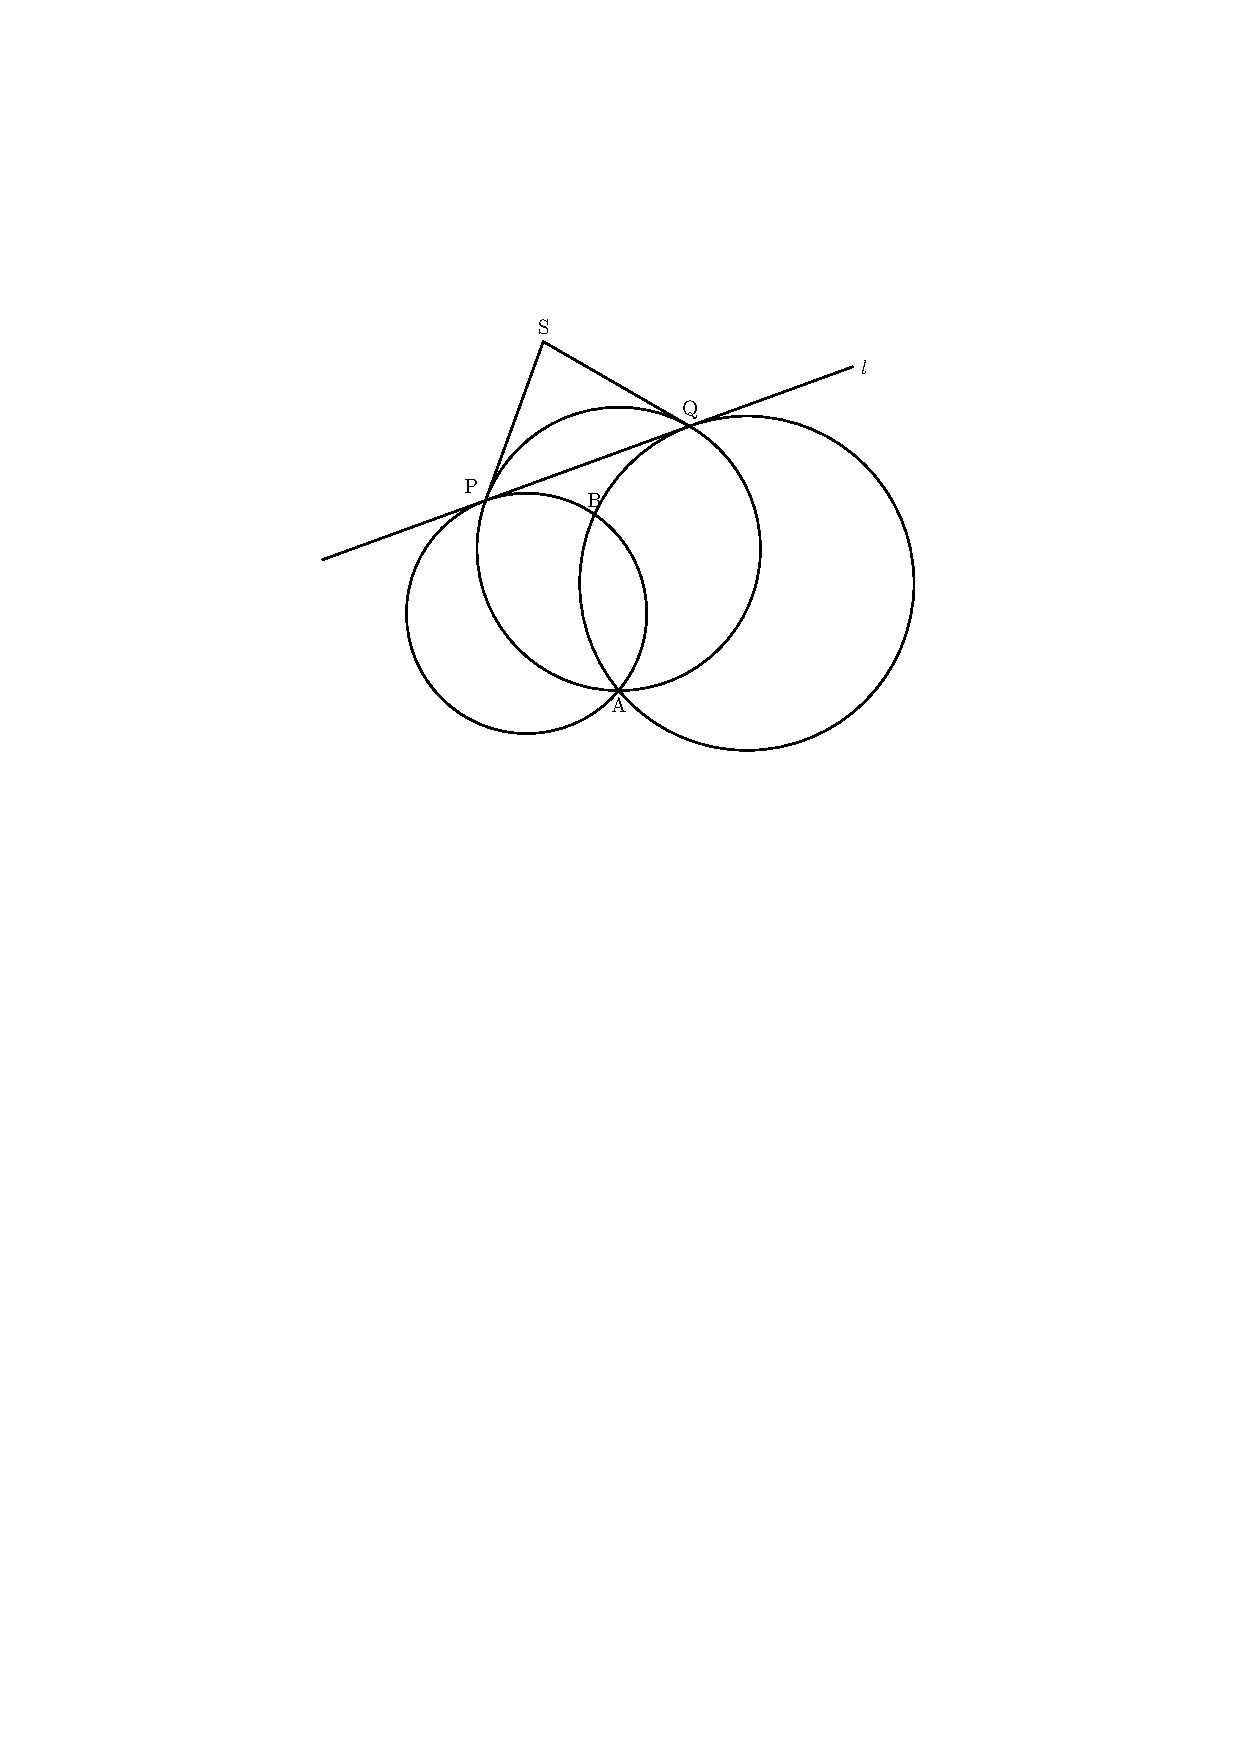
\includegraphics[width=8.0cm]{toujitsu_7_problem.pdf}
\end{figure}









\newpage

\section*{数学オリンピックワークショップ 当日問題G ---解答---}

\fbox{G6}

OBに関するQの対称点をQ$'$とすると,$\angle {\rm AOP} = \angle {\rm BOQ} = \angle {\rm BOQ'}$より,$\angle {\rm POQ'} = 90^{\circ}$となるので,$\triangle{\rm OPQ'}$は直角二等辺三角形。

ゆえに,$\rm PX+QX = PX+Q'X$は P, X, Q$'$が同一直線上にあるとき,最小値$6\sqrt 2$をとる。
\begin{figure}[ht]
  \centering
  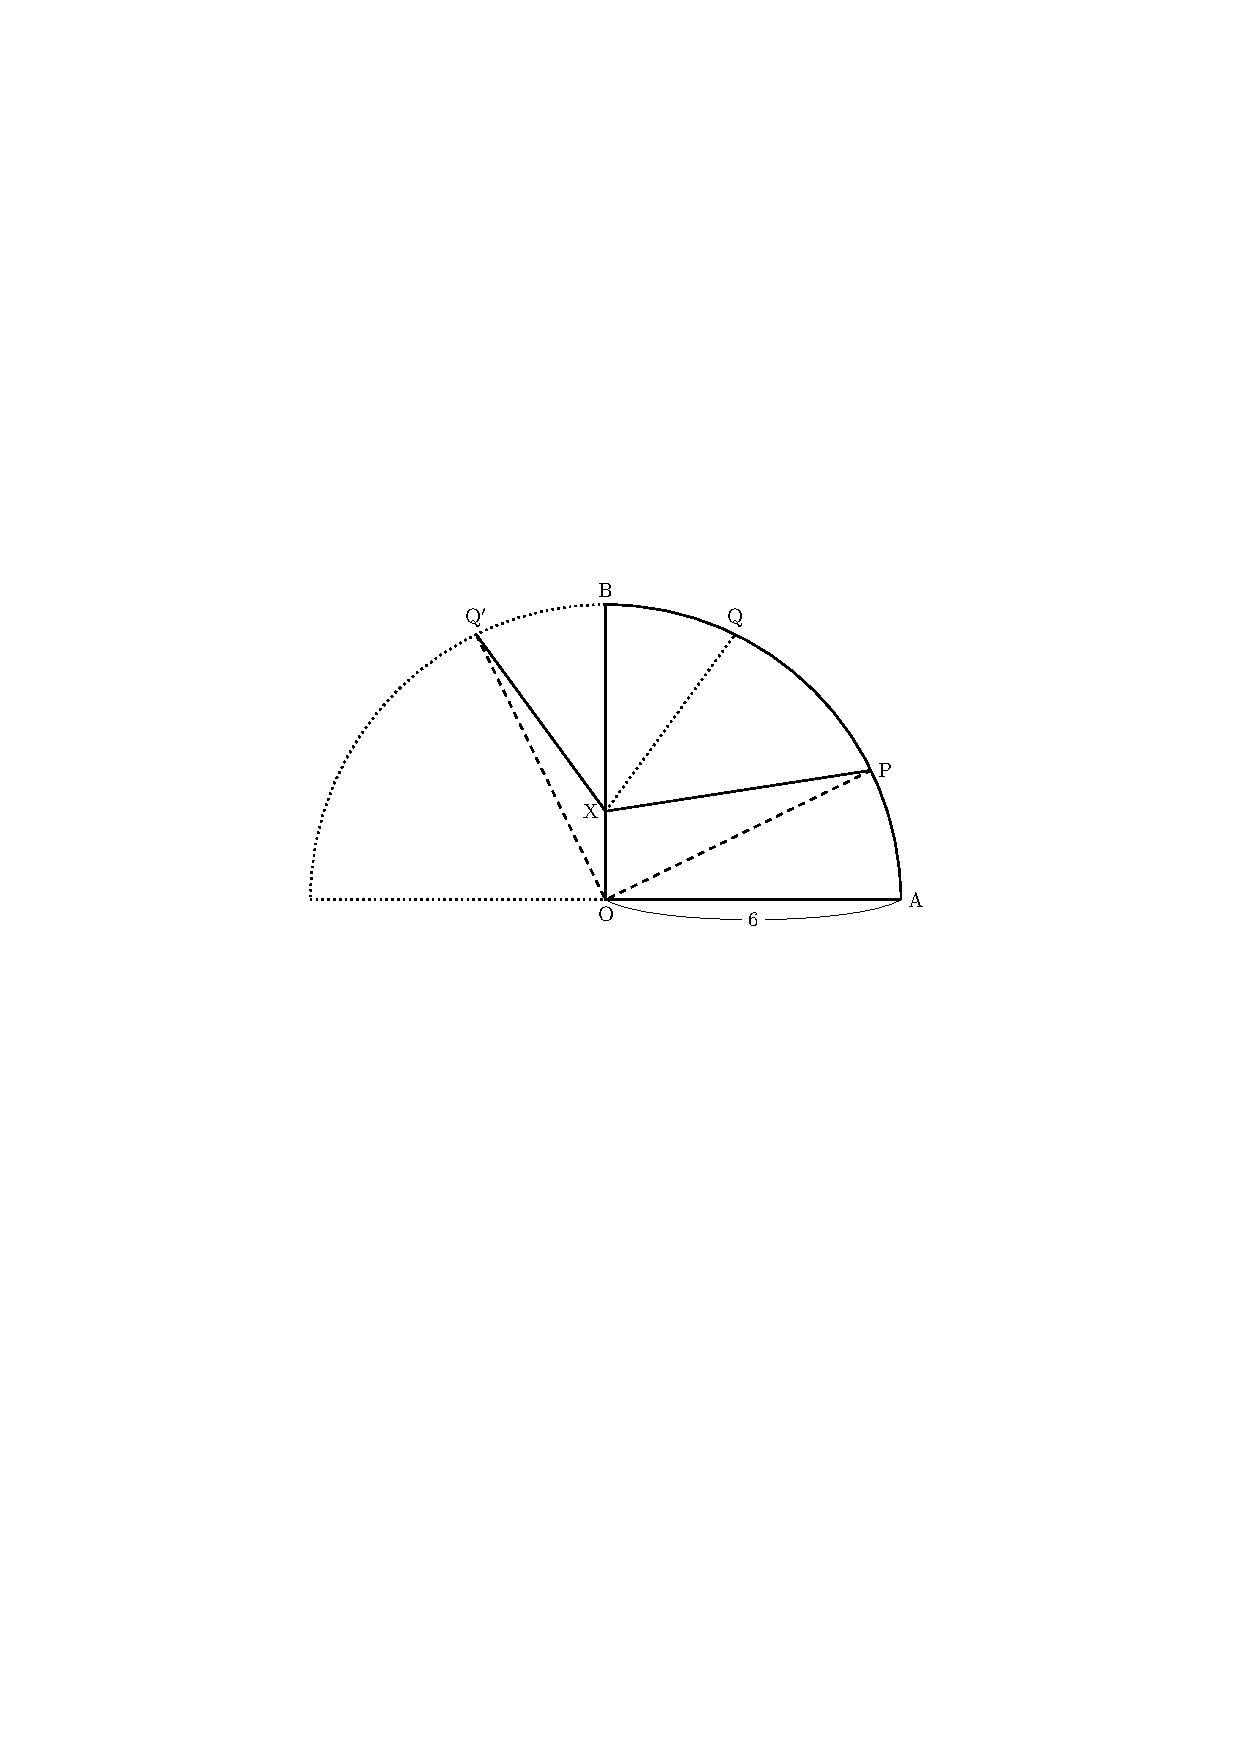
\includegraphics[width=9.0cm]{toujitsu_6_solution.pdf}
\end{figure}


\fbox{G7} 

ABと$l$の交点をMとすると方べきの定理より,
\begin{eqnarray*}
{\rm MP}^{2} &=& {\rm MB}\cdot {\rm MA}\\
&=& {\rm MQ}^{2}\\
\end{eqnarray*}
よって${\rm MP} = {\rm MQ}$,つまりMはPQの中点。

\begin{figure}[ht]
  \centering
  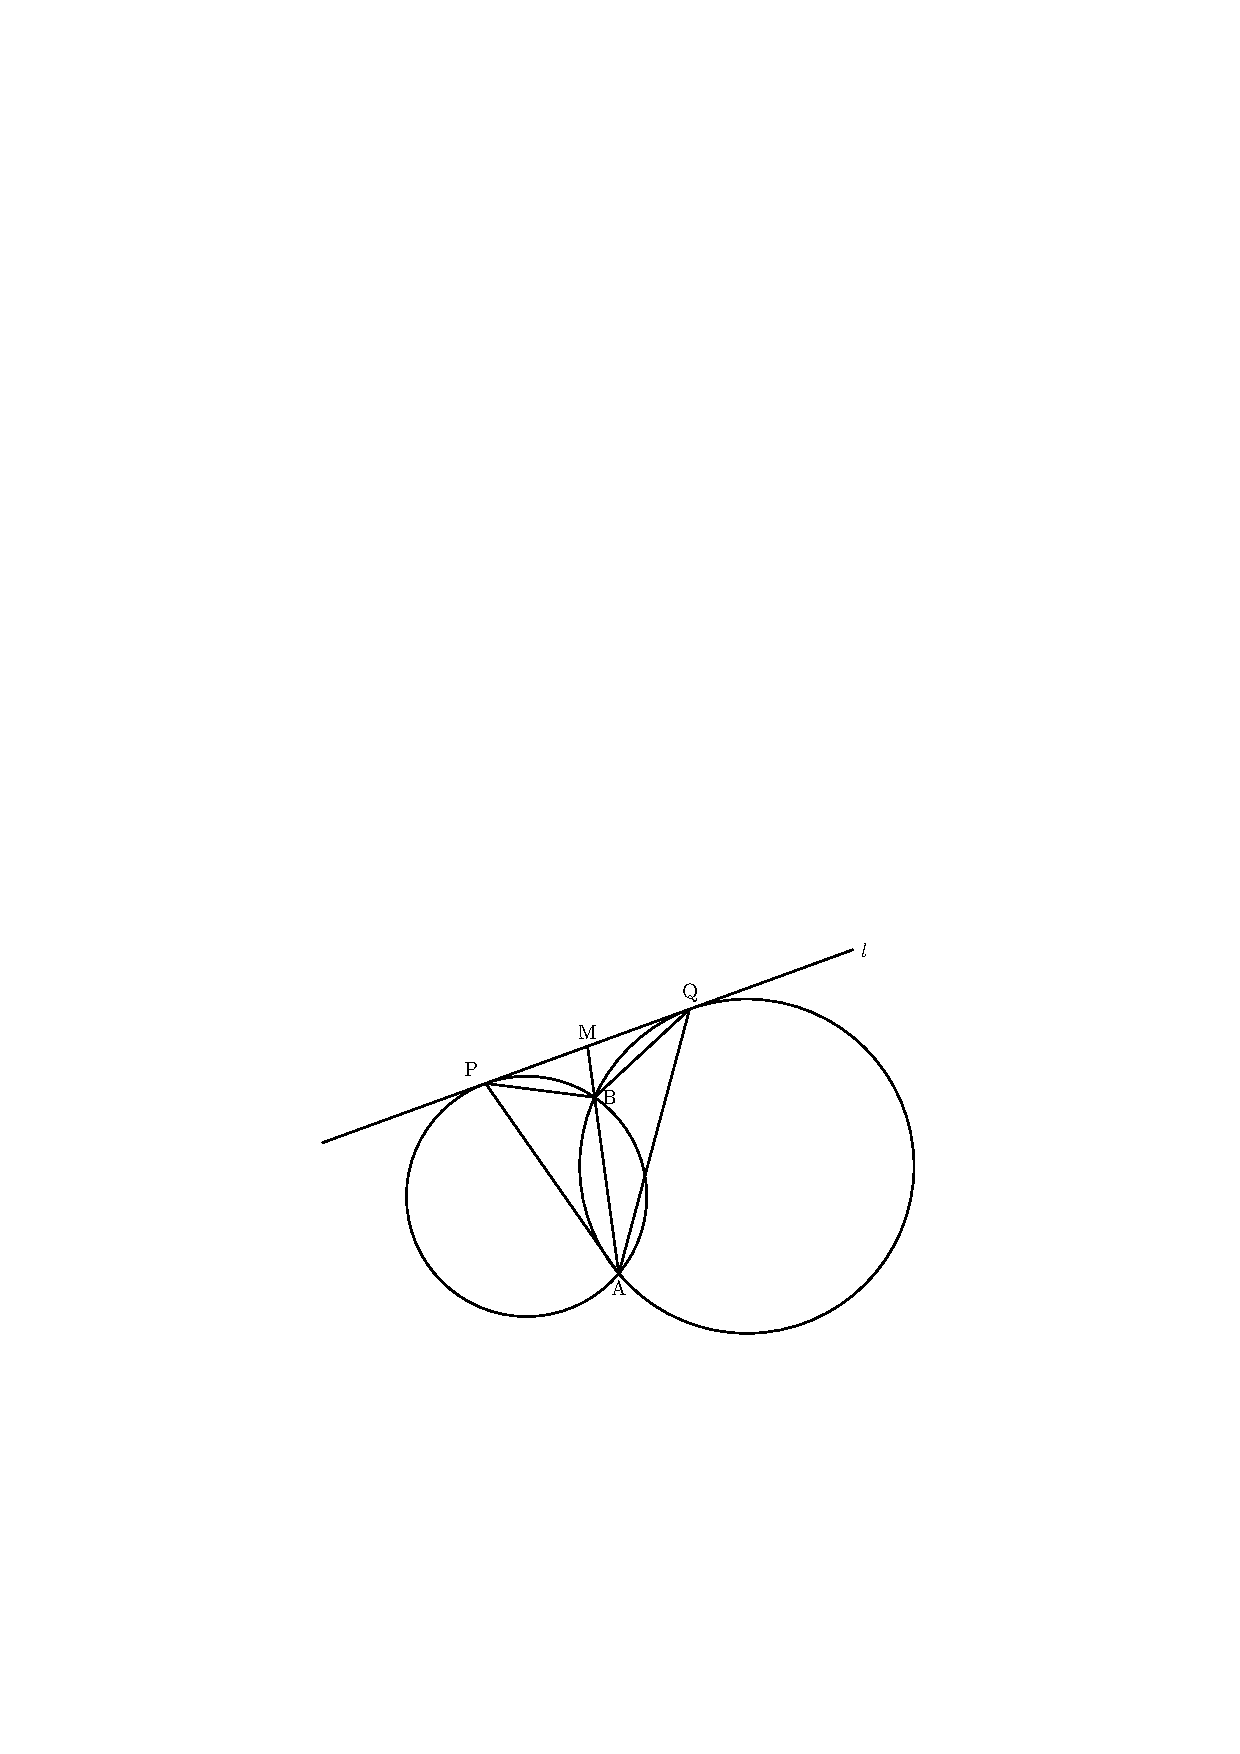
\includegraphics[width=9.0cm]{toujitsu_7_solution_1.pdf}
\end{figure}

\newpage

ゆえに,ASと$\triangle{\rm PAQ}$の外接円の交点をRとすれば,
\begin{align*}
&&&&\angle{\rm PQB} &= \angle{\rm QAM}   &&(\because \ 接弦定理)&&&&\\
&&&&                &= \angle{\rm PAS}   &&(\because \ \fbox{G5}(1))&&&&\\
&&&&                &= \angle{\rm PQR}   &&(\because \ 円周角の定理)&&&&
\end{align*}

同様に,$\angle{\rm QPB} = \angle{\rm QPR}$もわかるので,$\triangle{\rm BPQ} \equiv \triangle{\rm RPQ}$。つまり,$\rm B'$はRに他ならないので,$\rm A, B'=R, S$は同一直線上にある。
\begin{figure}[ht]
  \centering
  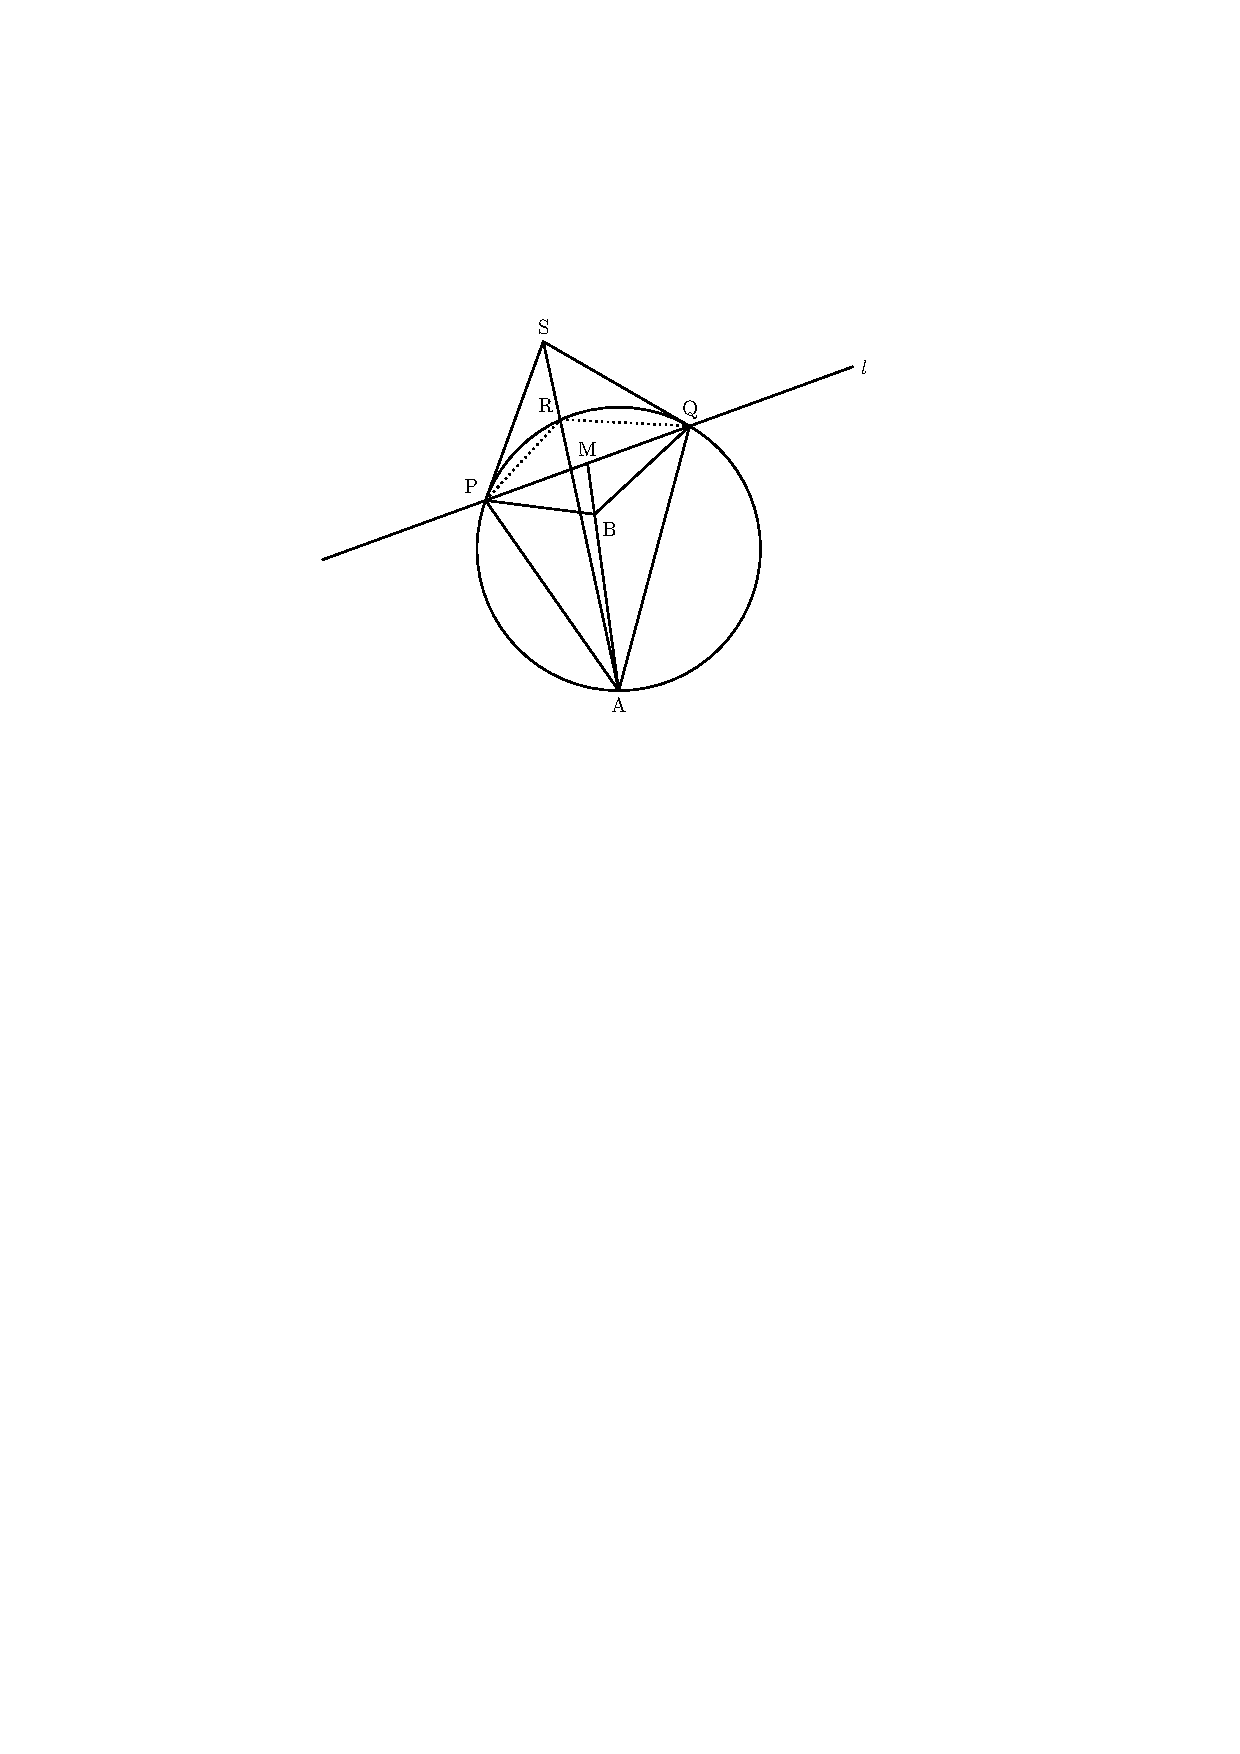
\includegraphics[width=9.0cm]{toujitsu_7_solution_2.pdf}
\end{figure}


\end{document}

